\documentclass[11pt,oneside]{article}
\usepackage[T1]{fontenc}
\usepackage[utf8]{inputenc}
\usepackage{lmodern}
\usepackage{microtype}
\usepackage[margin=1in]{geometry}
\usepackage{amsmath,amssymb,amsthm,mathtools}
\usepackage{booktabs,longtable,tabularx,array}
\usepackage{enumitem}
\usepackage{xcolor}
\usepackage{listings}
\usepackage{xurl}
\usepackage{hyperref}
\usepackage{fancyhdr}
\usepackage{lastpage}
\usepackage{makecell}
\usepackage{tikz}
\usetikzlibrary{arrows.meta,positioning,fit}

\definecolor{linkblue}{RGB}{30,74,120}
\definecolor{codegray}{RGB}{246,247,249}
\definecolor{darkgreen}{RGB}{30,100,60}
\hypersetup{
  colorlinks=true,
  linkcolor=linkblue,
  citecolor=linkblue,
  urlcolor=linkblue,
  pdftitle={Native Clause Programs for iPRA},
  pdfauthor={OpenAI, prepared for Vladimir Reshetnikov}
}
\setlength{\parindent}{0pt}
\setlength{\parskip}{0.58em}
\setlength{\emergencystretch}{3em}
\setlist{nosep,leftmargin=2em}
\setlength{\headheight}{14pt}
\pagestyle{fancy}
\fancyhf{}
\lhead{Native Clause Programs}
\rhead{Mathematics in iPRA}
\cfoot{\thepage\ of \pageref{LastPage}}
\renewcommand{\headrulewidth}{0.4pt}

\lstdefinestyle{lean}{
  basicstyle=\ttfamily\small,
  backgroundcolor=\color{codegray},
  frame=single,
  framerule=0.3pt,
  breaklines=true,
  columns=fullflexible,
  keepspaces=true,
  showstringspaces=false,
  tabsize=2
}
\lstset{style=lean}

\newtheorem{theorem}{Theorem}[section]
\newtheorem{lemma}[theorem]{Lemma}
\newtheorem{proposition}[theorem]{Proposition}
\newtheorem{corollary}[theorem]{Corollary}
\newtheorem{principle}[theorem]{Principle}
\newtheorem{barrier}[theorem]{Barrier}
\theoremstyle{definition}
\newtheorem{definition}[theorem]{Definition}
\newtheorem{construction}[theorem]{Construction}
\newtheorem{example}[theorem]{Example}
\newtheorem{remark}[theorem]{Remark}

\newcommand{\N}{\mathbb N}
\newcommand{\Z}{\mathbb Z}
\newcommand{\Q}{\mathbb Q}
\newcommand{\R}{\mathbb R}
\newcommand{\ipra}{\mathrm{iPRA}}
\newcommand{\PRAAx}{\mathsf{PRAAx}}
\newcommand{\Prf}{\mathsf{Prf}}
\newcommand{\KPrf}{\mathsf{KPrf}}
\newcommand{\NPrf}{\mathsf{NPrf}}
\newcommand{\Cl}{\mathsf{Cl}}
\newcommand{\NFm}{\mathsf{NFm}}
\newcommand{\PTm}{\mathsf{PTm}}
\newcommand{\Obs}{\mathsf{Obs}}
\newcommand{\Good}{\mathsf{Good}}
\newcommand{\Demand}{\mathsf{Demand}}
\newcommand{\Valid}{\mathsf{Valid}}
\newcommand{\diam}{\operatorname{diam}}
\newcommand{\rank}{\operatorname{rk}}
\newcommand{\code}{\operatorname{code}}
\newcommand{\height}{\operatorname{ht}}
\newcommand{\join}{\mathbin{\vee}}
\newcommand{\defeq}{\mathrel{:=}}
\newcommand{\pathcode}[1]{\texttt{#1}}
\newcolumntype{L}[1]{>{\raggedright\arraybackslash}p{#1}}

\title{\textbf{Native Clause Programs for iPRA}\\[0.35em]
\large A General Proof-Producing Framework for Embedding Mathematical Concepts and Arguments}
\author{Research report prepared for Vladimir Reshetnikov}
\date{15 November 2026 (America/Los\_Angeles)}

\begin{document}
\maketitle

\begin{center}
\fbox{\begin{minipage}{0.93\textwidth}
\textbf{Formal status.}
The mathematical arguments in this report are human proofs.  The source audit is
pinned to ProveIt commit
\path{8649990597d73657bde480b6c389de7f85bc0cb0}.  The report reuses Lean theorems
already present in \path{ConciseIPRA}, including the clause calculus \path{KPrf},
its substitution and cut theorems, its translation to \path{NPrf}, and the
native/iPRA equivalence.  It also incorporates the newly checked
\path{IPRADerivations} arithmetic and ring backend.  The accompanying Lean files
are an integration-oriented outline; no Lean executable was available in the
artifact environment, so no new theorem in this package is claimed to have been
kernel-checked.  The exact Python tests are regression evidence for finite
algorithms only, not proofs in iPRA.
\end{minipage}}
\end{center}

\begin{abstract}
The ProveIt collection contains dozens of detailed finitary reconstructions of
mathematical arguments, together with several general frameworks based on finite
observations, contracts, demand propagation, relational witnesses, and stable
observables.  The persistent gap is now sharply identifiable: a terminating
algorithm or a host-level Lean theorem is not yet an object-language derivation
\[
             \Prf\;\PRAAx\;[]\;\Phi.
\]
This report proposes a general framework that targets the repository's
kernel-checked five-rule clause calculus \(\KPrf\) as an intermediate proof
language.  A mathematical development is compiled into a finite \emph{native
clause program}: every node exports a quantifier-free native formula or clause,
every edge is an explicit finite dependency, and every node carries a local
\(\KPrf\) derivation.  Program composition is then not justified by semantic
reflection; it is ordinary \(\KPrf\) cut.  Parameter specialization is ordinary
\(\KPrf\) substitution.  The checked map \(\KPrf\to\NPrf\) followed by
\path{native_iff_pra} exports the result to ordinary iPRA.  Conversely, checked
\(\Prf\;\PRAAx\) derivations---notably the new polynomial identity backend in
\path{IPRADerivations}---can be imported as native clause nodes.

The report develops full human proofs of the compiler theorem, bounded trace
reflection, least bounded search, acyclic backward demand propagation, bounded
least fixed points for cyclic precision constraints, relational viability,
stable-observer elimination of noncanonical witnesses, exact recovery under a
positive gap, finite exceptional-set synchronization, lexicographic descent
fuel, and the equivalence between an explicit code-height bound and complete
finite enumeration.  It gives reusable presentations for integers, rationals,
represented reals and complex numbers, finite algebraic structures, matrices,
polynomials, simplicial data, and finite categories.  Representative
applications explain how the method handles polynomial identities,
fixed-dimensional Cayley--Hamilton, numerical analysis with moduli, root
clusters, spectral labels, finite topology, and conditional Diophantine
arguments.

The framework resolves several recurring repository difficulties: hidden host
computation, substitution bookkeeping, graph composition, changing precision,
cyclic resource requirements, and unstable witness selection.  It does not
manufacture absent deep quantitative producers.  General effective height
bounds, uniform Mordell--Weil covering representatives, ineffective
prime-distribution constants, and singular exact branch selectors remain
explicit interfaces rather than being renamed as certificates.
\end{abstract}

\section*{Executive conclusions}

The central recommendation is to standardize future developments on a
\emph{two-backend proof pipeline}.

\begin{enumerate}[label=\textbf{E\arabic*.}]
\item \textbf{Use ordinary \(\Prf\;\PRAAx\) for domain algebra.}
The new \path{IPRADerivations} library already supplies checked arithmetic,
semiring, integer, and polynomial-identity infrastructure.  A ring identity
should be proved there rather than reimplemented inside every packet.

\item \textbf{Use \(\KPrf\) for finite control and composition.}
The clause calculus is closed under substitution and has a proved cut theorem.
It is therefore a better intermediate representation for bounded loops,
search, finite branching, and proof graphs than an ad hoc host structure whose
soundness is still to be formalized.

\item \textbf{Compile concrete syntax, not encoded programs.}
A theorem-specific finite graph is specialized to actual terms, formulas, and
proof constructors before it is internalized.  No total primitive-recursive
universal evaluator and no truth-to-provability reflection principle is used.

\item \textbf{Keep relations when selection is unstable.}
Approximate roots, local charts, spectral subspaces, and compatible finite
models are represented by finite witness clouds.  A selector is introduced only
when bounded viability is needed; branch-independent information is extracted
by a stable observer without pretending that a canonical witness exists.

\item \textbf{Make quantitative producers visible.}
A search cutoff, convergence modulus, denominator bound, separation gap,
finite-cover certificate, or height bound is part of the theorem statement or
is produced by a separately proved node.  A cardinality statement is not a
search bound, and a terminating metaprogram is not an iPRA derivation.
\end{enumerate}

The package includes a dependency-ordered Lean plan, candidate bridge code,
exact finite reference algorithms, fourteen passing regression tests, a theorem
ledger, and a difficulty matrix.  The intended first implementation milestone
is small: kernel-check the list-cut and graph-fold layer against current
\path{NativeClausalDiagonal.lean}; then connect one existing
\path{IPRADerivations} polynomial theorem and one bounded trace example through
the complete import--compile--export route.

\tableofcontents
\clearpage
\section{Repository audit and the actual remaining layer}

\subsection{Pinned source baseline}

The audit was made against ProveIt commit
\path{8649990597d73657bde480b6c389de7f85bc0cb0}.  The relevant directory has
three logically different strata.

\begin{enumerate}
\item \path{ConciseIPRA} is a kernel-checked formalization of a small native
calculus, an equality calculus, and ordinary iPRA, together with
bi-interpretations.
\item \path{docs/proofs} is a large research corpus.  The packets contain
human proofs, code, and Lean plans, but the repository explicitly records that
they were filed without rerunning or checking them.
\item \path{Derivations} is a new checked library of actual
\(\Prf\;\PRAAx\) derivations.  Its first domain backend develops arithmetic,
a quotient semiring, integer differences, and a ring tactic, and applies them
to triangle identities.
\end{enumerate}

The distinction matters.  A packet may contain a correct mathematical
argument, a tested exact program, and a native Lean theorem while still lacking
a term of the type demanded by the embedded calculus.  The present framework
is designed to turn local embedded derivations into larger embedded
derivations; it does not reclassify evidence from one stratum as evidence in
another.

\subsection{What the earlier frameworks established}

The most mature foundation packets converge on a strong common discipline.
Infinite mathematical objects are accessed through finite observations;
algorithms declare backward precision demands; recursion is bounded and carries
a quantifier-free invariant; nonunique witnesses may be retained as finite
relations; and final exact branching is guarded by an apartness or gap
certificate.  PCOG and PFIG further formulate finite proof graphs and propose
compilers that fold local proofs in topological order.  OCiPRA classifies
statements into deterministic, relational, stable-observable, and conditional
producer forms.

These are substantial achievements.  The issue is not that another vocabulary
for ``certificate'' is needed.  The issue is that the generic compiler layer in
those packets is predominantly a blueprint.  In particular, many constructions
end at one of the following levels:

\begin{itemize}
\item a host function is proved correct as a function on natural numbers;
\item an exact Python program accepts all supplied examples;
\item a Lean structure contains a field whose type is the required derivation;
\item a local loop lemma is stated, but the substitutions, contexts, and cuts
needed to compose an application are left open;
\item a semantic theorem is proved about the interpretation of a formula, but
no derivation of the formula is built.
\end{itemize}

The new observation in this report is that current \path{ConciseIPRA} already
contains an intermediate proof language tailored to remove much of that work.

\subsection{The native clause calculus as an overlooked compiler IR}

A clause in \path{NativeClausal.lean} is a pair
\[
  [A;y.B(y)] \quad\text{read as}\quad A\to\forall y\,B(y).
\]
The calculus \(\KPrf\) has equation formulas and the native \(D\)-binder, and
five rule families: reflexivity, two evaluation cases, clause use, elimination,
and introduction.  The checked library proves, among other facts,
\[
\begin{aligned}
&\KPrf.\mathsf{subst},\qquad
  \KPrf.\mathsf{cut},\qquad
  \KPrf.\mathsf{toNPrf},\\
&\mathsf{kprf\_iff\_nprf},\qquad
  \mathsf{kprf\_iff\_nprf\_of\_qfree},\qquad
  \mathsf{native\_iff\_pra}.
\end{aligned}
\]
Thus the two operations that dominate a proof-graph compiler---specializing a
local theorem and discharging already proved dependencies---are not new
metatheorems to be built from scratch.  They are checked operations of the
intended object-level proof system.

This changes the recommended architecture.  Instead of defining a rich host
record \path{Contract} and later proving that every record field can be turned
into a derivation, we use an actual \(\KPrf\) derivation as the proof-carrying
field from the beginning.  A compiler fold then produces a larger \(\KPrf\)
derivation by cut.  Only at the boundary is the checked bridge to ordinary iPRA
applied.

\subsection{The new direct derivation backend}

The current \path{IPRADerivations} library fills another repeated gap.  Its
\path{Core/Basic.lean} supplies concrete primitive-recursive symbols for
addition, multiplication, predecessor, and truncated subtraction, together
with their equations, congruence rules, open quantifier-free induction
\path{ind}, and instantiation \path{inst}.  The subsequent files construct a
cancellative semiring of terms modulo provable equality, a ring of integer
differences, and the tactic \path{ipra_ring}.  The result of the tactic is not
merely a Mathlib equality: it is a derivation in \(\Prf\;\PRAAx\).

Accordingly, the present framework has two mutually connected backends:

\begin{center}
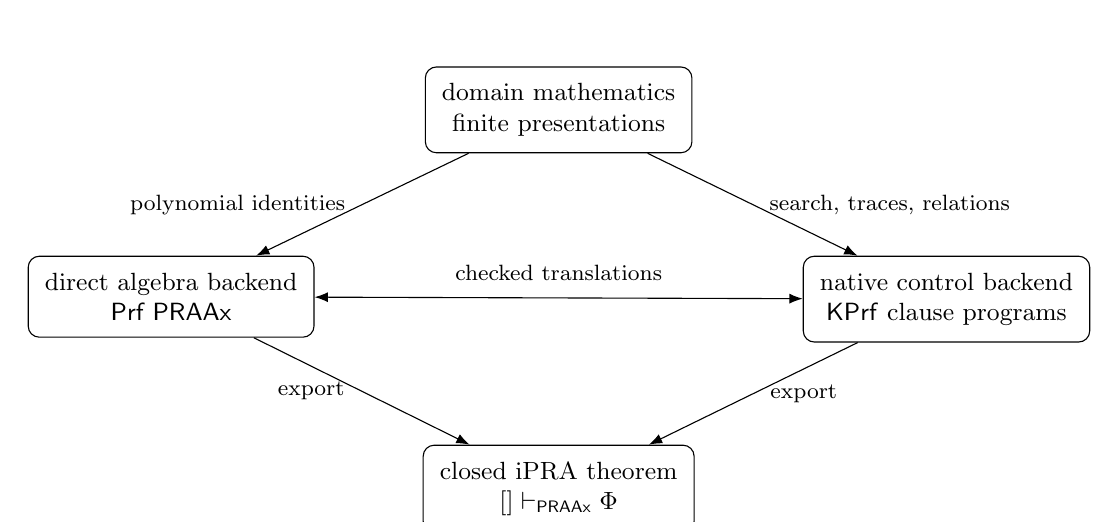
\begin{tikzpicture}[
  every node/.style={draw,rounded corners,align=center,inner sep=6pt,font=\small},
  every edge quotes/.style={draw=none,font=\footnotesize}, >=Latex]
\node (math) {domain mathematics\\finite presentations};
\node (pra) [below left=13mm and 14mm of math] {direct algebra backend\\$\Prf\;\PRAAx$};
\node (k) [below right=13mm and 14mm of math] {native control backend\\$\KPrf$ clause programs};
\node (out) [below=37mm of math] {closed iPRA theorem\\$[]\vdash_{\PRAAx}\Phi$};
\draw[->] (math) -- node[left,draw=none,font=\footnotesize]{polynomial identities} (pra);
\draw[->] (math) -- node[right,draw=none,font=\footnotesize]{search, traces, relations} (k);
\draw[<->] (pra) -- node[above,draw=none,font=\footnotesize]{checked translations} (k);
\draw[->] (pra) -- node[left,draw=none,font=\footnotesize]{export} (out);
\draw[->] (k) -- node[right,draw=none,font=\footnotesize]{export} (out);
\end{tikzpicture}
\end{center}

A polynomial identity should go through the first backend.  A bounded search,
finite branch tree, demand scheduler, or relational observer should go through
the second.  A theorem may use both.

\subsection{Recurring failure modes}

The source audit identifies nine recurring failure modes that a general
framework must address explicitly.

\begin{longtable}{L{0.25\textwidth}L{0.66\textwidth}}
\toprule
Failure mode & Required repair \\
\midrule
Host correctness only & Carry an actual \(\KPrf\) or \(\Prf\;\PRAAx\) local proof and compose it in the embedded calculus.\\
Universal evaluator assumption & Specialize each fixed finite program to concrete primitive-recursive syntax before internalization.\\
Hidden precision choices & Propagate an explicit demand vector backward; for cycles compute a bounded least fixed point.\\
Unstable exact selector & Keep a finite relation or cloud and extract only a stable observation.\\
Approximate equality used as exact equality & Require a positive gap or retain an error-bearing statement.\\
Cardinality used as cutoff & Require a code-height bound or a complete finite list.\\
Classical compactness used silently & Replace it by a finite cover, finite subcover certificate, or metastable finite window.\\
Deep producer renamed ``certificate'' & State the producer as a separate interface and prove only the verifier and compiler generically.\\
One large theorem with unclear status & Maintain a theorem ledger separating human proof, executable check, Lean outline, and kernel-checked derivation.\\
\bottomrule
\end{longtable}

\subsection{Objective of the present report}

The objective is not to assert that all mathematics is primitive recursive in
an unqualified sense.  It is the following conditional but useful compiler
theorem.

\begin{principle}[Native proof-producing compilation]
For a fixed mathematical construction, suppose all ideal objects are replaced
by finite observations; all searches, loops, and branch sets have explicit
bounds; all non-total operations are guarded by certificates; and every local
operation carries a derivation in either the native clause calculus or ordinary
iPRA.  Then the finite dependency graph can be compiled, by checked
substitution and cut, into an ordinary iPRA derivation of its exported finite
contract.
\end{principle}

The statement deliberately has hypotheses.  Those hypotheses are where a deep
mathematical theorem contributes its effective content.  The value of the
framework is that, once the content is present, the remaining encoding,
resource accounting, finite search, and proof composition are uniform.

\section{The target theory and nonnegotiable constraints}

\subsection{What counts as an iPRA theorem}

The ordinary target has terms built from primitive-recursive symbols and
formulas of intuitionistic first-order logic with equality.  Its arithmetic
axioms are the defining equations for those symbols, the successor axioms, and
induction restricted to quantifier-free formulas.  In the repository the
judgment is represented by
\[
       \Gamma\ \vdash_{\PRAAx}\ \varphi,
\]
that is, a term of the inductive type \(\Prf\;\PRAAx\;\Gamma\;\varphi\).
A closed theorem therefore ends at a concrete type
\[
       ([]:\mathrm{List}(\mathrm{Fm}\;\PTm\;0))
           \ \vdash_{\PRAAx}\ \Phi.
\]
A proof in ordinary Lean of the semantic proposition represented by \(\Phi\)
is valuable but is not the same object.

The native scalar core is a smaller, bi-interpretable presentation.  Native
terms have an iterator; native formulas are equations and two binders \(Q,D\).
The theorem \path{native_iff_pra} states the exact equivalence between native
derivability and derivability of the ordinary reading.  This permits the
compiler to work in the clause-friendly native language without changing the
ultimate theory.

\subsection{Induction discipline}

Only quantifier-free induction is primitive.  Consequently every recursive
proof must expose a quantifier-free state invariant.  Quantified mathematical
content can still occur in the theorem, but it must not be hidden in the
induction formula.  There are three standard repairs.

\begin{enumerate}
\item Replace a bounded quantified assertion by a characteristic primitive-
recursive term and induct on the equation saying that the characteristic value
is one.
\item Store all witnesses needed up to time \(t\) in one coded finite state, so
that the invariant is a quantifier-free predicate of that state.
\item Prove the recursive computational lemma quantifier-freely first and apply
ordinary logical rules only after the recursion has terminated.
\end{enumerate}

This ``compute first, quantify later'' separation is not merely stylistic.  It
prevents a common invalid argument in which a perfectly ordinary induction in
Heyting arithmetic is assumed to be available in iPRA.

\subsection{No universal primitive-recursive interpreter}

The class of primitive-recursive functions is effectively enumerable, but a
total primitive-recursive evaluator for arbitrary encoded primitive-recursive
programs cannot exist with the expected universal property: diagonalization
would produce a primitive-recursive function outside the enumeration.  A
generic framework must therefore not postulate a term
\(\mathsf{eval}(e,x)\) that internally executes every encoded PR program.

The permitted compiler is staged.  At the host level it receives a fixed finite
program graph and constructs concrete syntax for each primitive-recursive
operation in that graph.  The generated object theorem concerns those concrete
symbols.  Genericity belongs to the host theorem about the compiler; execution
inside iPRA remains theorem-specific syntax.

\subsection{Finite use rather than completed infinity}

A real number, function, space, group, sheaf, probability law, or category is
not inserted into first-order arithmetic as a new set-theoretic object.  It is
presented by codes for finite observations and laws governing those
observations.  A theorem must specify which finite observations it consumes for
a requested output observation.

For example, a represented real \(x\) is accessed through a primitive-
recursive rational name \(a_x(q)\) and a modulus statement such as
\[
       |a_x(q)-x|\le 2^{-q}.
\]
Inside the arithmetic theorem, the ideal symbol \(x\) is normally absent.  The
actual statement compares rational codes at explicit precisions.  The ideal
real appears only in the external adequacy theorem explaining the intended
meaning of the representation.

\subsection{Guarded partial operations}

Division, normalization, chart inversion, root labeling, and elimination of a
pivot are not total operations on codes.  They become total primitive-
recursive operations on a larger input containing a guard.  Typical guards are
\[
   |d|\ge 2^{-g},\qquad \det M\ne0,\qquad
   \diam C\le 2^{-q},\qquad \operatorname{dist}(A,B)\ge\delta>0.
\]
The computational function may return a default value when the guard fails;
the local proof contract states correctness under the guard.  This is the
correct way to reconcile total primitive recursion with mathematically partial
operations.

\subsection{Intuitionistic existence and data}

An existential theorem in an intuitionistic calculus carries evidence, but the
form of that evidence may be relational rather than a globally canonical
function.  If a bounded finite cloud has at least one valid witness, bounded
least search can choose one.  If compatibility through all precisions is only
known relationally, a finite-horizon path can be selected for each requested
horizon.  If the desired output is invariant across all witnesses, no selector
is needed at all.

The framework therefore distinguishes:

\begin{itemize}
\item \emph{deterministic producer}: computes one certified code;
\item \emph{bounded relation}: computes a finite set of certified codes;
\item \emph{stable observer}: computes information common to all certified
codes up to a stated error;
\item \emph{conditional producer}: accepts nonuniform quantitative data as an
explicit theorem hypothesis.
\end{itemize}

Collapsing these classes is a source of false uniformity claims.

\subsection{Statement-design checklist}

Before formalization, every headline theorem should pass the following test.

\begin{enumerate}
\item Every ideal object has a fixed numerical presentation.
\item Every finite structure has an explicit code bound or coded list.
\item Every analytic output has a rational tolerance and a modulus or
certificate from which the required input precision is computed.
\item Every recursive component has a clock and a quantifier-free invariant.
\item Every search has a cutoff with recorded provenance.
\item Every exact comparison has decidable coded data or an apartness witness.
\item Every nonunique intermediate is either kept relational or eliminated by
an observer-stability theorem.
\item Every deep nonuniform input is visible in the theorem interface.
\item The final endpoint is written as a concrete \(\KPrf\), \(\NPrf\), or
\(\Prf\;\PRAAx\) type.
\end{enumerate}

A theorem that fails this checklist may still be mathematically true, but its
present form is not yet ready for iPRA compilation.

\section{Finite presentations and observation contracts}

\subsection{Presentations}

The framework starts before proof syntax.  A mathematical object must first be
replaced by a finite-use presentation.

\begin{definition}[Finitary presentation]
A finitary presentation \(X\) consists of primitive-recursive data
\[
 (\mathsf{Code}_X,\mathsf{Query}_X,\mathsf{Obs}_X,
   \mathsf{valid}_X,\mathsf{restrict}_X)
\]
with the following intended meanings.
\begin{enumerate}
\item \(x\in\mathsf{Code}_X\subseteq\N\) is a code or name for an input.
\item \(q\in\mathsf{Query}_X\) is a finite request: precision, radius, degree,
finite subdiagram, support bound, or resource level.
\item \(o\in\mathsf{Obs}_X(x,q)\) is a finite observation code.
\item \(\mathsf{valid}_X(x,q,o)\in\{0,1\}\) is a decidable validity predicate.
\item If \(q\preceq q'\), the restriction operation maps a valid observation at
\(q'\) to one at \(q\).
\end{enumerate}
All domains may be represented by natural-number bounds and characteristic
terms; the typed notation is explanatory.
\end{definition}

The coherence law is
\[
  q\preceq q'\preceq q'',\quad
  \mathsf{valid}(x,q'',o'')
  \quad\Longrightarrow\quad
  \mathsf{restrict}_{q'',q}(o'')
  =\mathsf{restrict}_{q',q}
      (\mathsf{restrict}_{q'',q'}(o'')).
\]
This law is an equation between PR terms or a bounded formula, hence suitable
for the object theory.  It prevents the presentation from offering unrelated
answers at different precisions.

A presentation need not have a unique observation.  This is essential.  An
algebraic number may be represented by an isolating disk; a root at a collision
may have several compatible disks; a compact space may have many finite nets;
a quotient object may have many representatives.  The validity relation is
therefore primary, and a deterministic name is a special case.

\subsection{Deterministic and relational names}

\begin{definition}[Deterministic name]
A deterministic name is a primitive-recursive function
\(a_X(x,q)\) with a proof of
\(\mathsf{valid}_X(x,q,a_X(x,q))\) and restriction coherence.
\end{definition}

\begin{definition}[Finite relational name]
A finite relational name supplies a primitive-recursive bound \(B_X(x,q)\) and
a validity predicate such that
\[
        \exists o\le B_X(x,q)\;\mathsf{valid}_X(x,q,o).
\]
The cloud at \(q\) is the finite set of all valid \(o\le B_X(x,q)\).
\end{definition}

The existential statement may itself be produced constructively, or it may be
a hypothesis supplied by a deep theorem.  Once the bound and validity relation
are available, complete enumeration, least search, and all universal checks
over the cloud are primitive recursive.

\subsection{Observation contracts}

An operation is specified by what it must observe, not by an unbounded semantic
function.

\begin{definition}[Deterministic observation contract]
A deterministic contract \(F:X\to Y\) consists of:
\begin{enumerate}
\item a backward demand transformer
\(d_F(x,r)\in\mathsf{Query}_X\);
\item a primitive-recursive transformer
\(f_F(x,r,o)\in\mathsf{Obs}_Y\);
\item a local proof that
\[
 \mathsf{valid}_X(x,d_F(x,r),o)
 \longrightarrow
 \mathsf{valid}_Y(Fx,r,f_F(x,r,o)).
\]
\end{enumerate}
The displayed implication is ultimately encoded as a native clause or ordinary
iPRA formula.
\end{definition}

\begin{definition}[Relational observation contract]
A relational contract replaces \(f_F\) by a finite output bound and relation
\(R_F(x,r,o,v)\).  Its local proof states that every valid demanded input
observation has at least one valid related output and that every related output
satisfies the advertised \(Y\)-contract.
\end{definition}

A contract is not a semantic assertion that a host function is continuous.  It
is a finite theorem: a particular input observation at a computed demand
suffices to verify a particular output observation.

\subsection{Composition of deterministic contracts}

Let \(F:X\to Y\) and \(G:Y\to Z\) be deterministic contracts.  For a requested
query \(s\) on \(Z\), first compute the \(Y\)-query
\(r=d_G(Fx,s)\), then the \(X\)-query
\[
     d_{G\circ F}(x,s)=d_F(x,r).
\]
Given an observation \(o\) at this demand, form
\[
   u=f_F(x,r,o),\qquad v=f_G(Fx,s,u).
\]
The local proof for \(F\) gives validity of \(u\), and the local proof for
\(G\) gives validity of \(v\).  In the proof compiler the corresponding
operation is cut.

\begin{theorem}[Deterministic contract composition]
Deterministic observation contracts are closed under identity and composition.
Demand transformers and realizers remain primitive recursive, and local
object-language proofs compose by cut.
\end{theorem}

\begin{proof}
The identity demand is the requested query and the identity realizer is
restriction or literal identity.  For composition, the formulas above are
primitive-recursive compositions.  The proof of the composite contract is the
first local derivation followed by the second, discharging the intermediate
validity formula.  The formal version is Theorem~\ref{thm:list-cut} below.
Associativity holds extensionally because primitive-recursive composition and
proof cut are associative up to derivability; no equality of proof terms is
needed.
\end{proof}

\subsection{Adaptive finite use}

Many algorithms do not know all input requests in advance.  A bisection routine
chooses its next interval from a sign test; a pivoting algorithm asks for a gap
after inspecting a candidate pivot; a continuation method changes precision
when an error estimate is large.  Such an algorithm is still finitely
presentable when it is clocked.

A state \(s_t\) contains both mathematical data and a finite request log.  At
step \(t\), a primitive-recursive rule computes the next query from \(s_t\),
reads the corresponding input observation, and produces \(s_{t+1}\).  For a
fixed fuel \(T\), the total demand is the maximum of the finitely many queries
recorded in the trace.  Rather than pretending that the adaptive algorithm is a
single nonadaptive contract, the framework compiles its trace and proves the
invariant that every query was answered correctly.

\subsection{Products, sums, subobjects, and quotients}

Finite presentations are closed under the ordinary constructions needed by
mathematics.

\paragraph{Products.}
A query for \(X\times Y\) is a pair of queries, an observation is a pair of
observations, and validity is conjunction.  Pairing functions code the pair by
a natural number.  Projections are exact PR operations.

\paragraph{Finite sums.}
An observation has a tag and a payload.  Validity checks the tag and invokes
the relevant component predicate.  Exact case analysis is permitted because
the tag is a decidable natural number.

\paragraph{Subobjects.}
A subpresentation is a presentation plus a decidable or explicitly certified
property.  The property is carried as part of validity.  For an open property,
one must decide whether the theorem uses it as a hypothesis or supplies a
finite certificate.

\paragraph{Quotients.}
A quotient should generally not choose canonical representatives.  It is
presented by representatives, a bounded equivalence relation on the demanded
finite data, and observers invariant under that relation.  A normal form may be
added when a primitive-recursive normalization theorem is available, but it is
not part of the general quotient interface.

\subsection{Adequacy without reflection}

Each presentation has an external adequacy theorem connecting its finite codes
to the intended mathematical object.  For represented reals, adequacy says
that a coherent rapidly Cauchy rational name determines a real.  For finite
simplicial complexes, the code decodes to an abstract complex.  For matrices,
the code decodes to a fixed finite table.

Adequacy is not used as a truth-to-provability rule.  The object theorem is
stated directly about codes and validity predicates.  Adequacy explains why
that theorem is the desired mathematical statement.  This separation permits
classical mathematics to be used in a metatheoretic interpretation without
silently importing classical axioms into the derivation.

\subsection{Producers, verifiers, and finalizers}

A recurring source of overclaim is failure to separate three roles.

\begin{definition}[Producer--verifier--finalizer factorization]
A theorem pipeline is factored as follows.
\begin{enumerate}
\item A \emph{producer} supplies candidate finite data and quantitative bounds.
It may be a primitive-recursive algorithm, an explicit theorem hypothesis, or a
separately established deep result.
\item A \emph{verifier} is a primitive-recursive bounded checker for the local
contract.
\item A \emph{finalizer} turns verified finite data into the stated output and
carries the object-language derivation of correctness.
\end{enumerate}
\end{definition}

The general framework proves closure of verifiers and finalizers.  It proves a
producer only when an actual mathematical construction and its quantitative
analysis are supplied.  In particular, saying ``let the certificate contain a
height bound'' does not prove a height bound.

\section{The native clause intermediate representation}

\subsection{Why clauses are the right granularity}

A proof graph repeatedly uses statements of the form
\[
       \text{when a finite precondition holds, every requested instance of a
       local invariant holds.}
\]
This is precisely the shape of a clause
\([A;y.B(y)]\), read \(A\to\forall y B(y)\).  In the checked Lean source the
structure is
\begin{lstlisting}[language={},caption={The upstream clause datatype, schematically}]
structure Cl (n : Nat) where
  ante : NFm n
  cons : NFm (n + 1)
\end{lstlisting}
The clause calculus stores such clauses in the context.  Its \path{use} rule
proves an instance \(B(t)\) after proving the antecedent \(A\).

A plain assumption \(X\) is represented by \path{Cl.asm X}, whose antecedent is
\(0=0\) and whose consequent is the shifted formula \(X\).  This representation
is important for program compilation: predecessor outputs are inserted as
ordinary assumption clauses, and \(\KPrf.\mathsf{cut}\) can discharge them with
already compiled proofs.

\subsection{Formula discipline}

The raw clause calculus is optimized for \(Q\)-free native formulas: equations
and the native \(D\)-binder.  Arbitrary native formulas are translated by
\path{NFm.unQ}, which rewrites \(Q_y B\) as a \(D\)-formula whose witness
coordinate is unused.  The checked theorems state
\[
\begin{aligned}
\KPrf(\Gamma^{\mathsf{asm}},A)&\iff\NPrf(\Gamma,A)
    &&\text{for \(Q\)-free sequents},\\
\KPrf((\mathsf{unQ}\,\Gamma)^{\mathsf{asm}},\mathsf{unQ}\,A)
    &\iff\NPrf(\Gamma,A)
    &&\text{in general}.
\end{aligned}
\]
Hence a compiler may normalize all exported node formulas to \(Q\)-free form
without loss of provability.

The native language has no primitive conjunction or implication, but this is
not a limitation on expressiveness: the scalar core defines the usual logical
connectives as macros and is bi-interpretable with ordinary iPRA.  At the
compiler level it is often simpler to split a conjunction into several node
outputs or package several equations into one coded Boolean equation.

\subsection{The five rule families}

The calculus has the following operations.

\begin{enumerate}
\item \textbf{Refl}: derive \(t=t\).
\item \textbf{Eval}: the two iterator computation cases, expressed so that an
existing equation about the counter and one about the iterator produce the
next equation.
\item \textbf{Use}: instantiate a clause after proving its antecedent.
\item \textbf{Elim}: open a \(D\)-formula at a fresh witness and continue under
the corresponding clause.
\item \textbf{Intro}: prove a \(D\)-formula from a progress derivation.  Its
start mode is read from the diagonal shape of the matrix.
\end{enumerate}

For framework design, the crucial checked derived operations are weakening,
renaming, substitution, and cut.  These operations are proved by structural
induction on \(\KPrf\) derivations.  Consequently, a proof compiler may treat
them as trusted library combinators rather than re-proving capture-avoidance and
context transport for every node class.

\subsection{Clause-carrying nodes}

\begin{definition}[Native clause node]
Fix a base clause context \(\Gamma\) and a list \(\Delta\) of predecessor
outputs, each a native formula with \(n\) free variables.  A native clause node
consists of:
\begin{enumerate}
\item an output formula \(A\in\NFm(n)\);
\item a proof that \(A\) is \(Q\)-free, or a prescribed \path{unQ}
normalization;
\item an actual local derivation
\[
   h:\KPrf\bigl(\Delta.\mathsf{map}(\Cl.\mathsf{asm})\mathbin{++}\Gamma,A\bigr);
\]
\item optional executable metadata: demand transformers, resource bounds,
trace descriptions, witness-cloud bounds, or observer tolerances.
\end{enumerate}
\end{definition}

The executable metadata does not justify the node.  The field \(h\) does.  The
metadata is used to generate concrete terms and to make the theorem auditable.

\subsection{Normalized node classes}

Most applications can be normalized to six classes.

\paragraph{Equation nodes.}
These export an equation between concrete PR terms.  Examples include tuple
projection, polynomial evaluation, finite table lookup, rational normalization,
substitution, and fixed-dimensional matrix multiplication.  Their proofs use
computation equations, congruence, and algebraic lemmas.

\paragraph{Clause nodes.}
These add reusable implications of the form \([A;y.B(y)]\).  They encode local
invariants, guarded operations, or universal finite families.  The antecedent
is a guard, not an invitation to use an undecidable partial function.

\paragraph{Trace nodes.}
A trace node contains an initializer, PR step, fuel, quantifier-free invariant,
base derivation, and step derivation.  It exports the terminal invariant or a
clause giving every bounded instance.

\paragraph{Search nodes.}
A search node contains a finite bound and a Booleanized predicate.  It exports a
least witness, a complete list, or the equation recording that no witness was
found.  Search correctness is a trace theorem.

\paragraph{Relational nodes.}
These export a finite witness cloud and compatibility edges.  They avoid
constructing a global selector.  Bounded viability may later select a path, or
a stable observer may eliminate the witness.

\paragraph{Finalizer nodes.}
A finalizer converts verified finite evidence into the exact headline formula.
It is the only place where theorem-specific logical packaging should occur.
Keeping finalization separate makes it clear which part of the development is
uniform and which part encodes the mathematical statement.

\subsection{Effects as data, not proof rules}

Each node may carry an effect record
\[
  (\text{precision},\text{fuel},\text{height},\text{denominator},
    \text{gap},\text{cover},\text{exception budget}).
\]
Effects are natural-number terms and finite certificates.  They guide the host
compiler and appear in contracts.  They are not new logical rules.  For
example, a gap effect is a formula proving a positive rational lower bound; a
height effect is a numeral or PR term bounding every candidate code; a cover
effect is a coded finite list together with a bounded covering check.

This design keeps the trusted proof kernel small while permitting a rich
application-level interface.

\subsection{No semantic reflection}

A native clause program is proof-producing in the literal sense: each node
contains a derivation.  The graph compiler never proves
``the checker returned true, therefore the formula is provable.''  It instead
constructs the formula's derivation from the node's local derivation and the
compiled predecessor derivations.  The checker may be used to generate or
validate data, but the proof term remains the authority.

This distinction is especially important for generated arithmetic.  A Python
program may confirm a million finite cases; unless the cases are compiled into
a bounded trace theorem or a closed proof term, that confirmation is not an
iPRA proof.  Conversely, a short \(\KPrf\) derivation may prove all cases even
when the reference program is present only for regression testing.

\section{The checked compiler spine}

\subsection{Simultaneous discharge of generated assumptions}

The central structural lemma is a finite list form of cut.  It is almost a
direct call to the checked theorem \path{KPrf.cut}.

\begin{theorem}[List cut]\label{thm:list-cut}
Let \(\Gamma\) be a base clause context, let
\(\Delta=[B_0,\ldots,B_{r-1}]\) be native formulas, and let \(A\) be a native
formula.  If
\[
  h:\KPrf(\Delta^{\mathsf{asm}}\mathbin{++}\Gamma,A)
\]
and for every \(B_i\in\Delta\) there is
\(h_i:\KPrf(\Gamma,B_i)\), then \(\KPrf(\Gamma,A)\).
\end{theorem}

\begin{proof}
Apply \path{KPrf.cut} to \(h\) with target context \(\Gamma\).  Every source
clause belongs either to \(\Gamma\), in which case it is retained, or to
\(\Delta^{\mathsf{asm}}\), in which case it has the form
\(\Cl.\mathsf{asm}(B_i)\) and is discharged by \(h_i\).  These are exactly the
two alternatives required by the checked cut theorem.  The argument is a
finite list-membership decomposition and does not inspect the internal
structure of \(h\).
\end{proof}

A candidate Lean proof is included in \path{lean/NativeClauseFramework/Bridge.lean}:

\begin{lstlisting}[language={},caption={Candidate direct proof of list cut}]
theorem cutAsmList
    (h : KPrf (Delta.map Cl.asm ++ Gamma) A)
    (hs : forall X, X in Delta -> KPrf Gamma X) : KPrf Gamma A := by
  apply h.cut
  intro c hc
  rw [List.mem_append] at hc
  rcases hc with hc | hc
  case left => obtain <X, hX, rfl> := List.mem_map.1 hc
    exact .inr <X, rfl, hs X hX>
  case right => exact .inl hc
\end{lstlisting}
The archive uses ASCII approximations in explanatory snippets where convenient;
the actual Lean file uses Lean syntax.

\subsection{Acyclic program compilation}

A program is given in topological order.  Node \(i\) may depend on any subset
of outputs \(A_0,\ldots,A_{i-1}\), and its local proof is allowed to assume all
previous outputs for simplicity:
\[
 h_i:\KPrf([A_0,\ldots,A_{i-1}]^{\mathsf{asm}}
                 \mathbin{++}\Gamma,A_i).
\]
Unused assumptions are harmless.

\begin{theorem}[Native DAG compilation]\label{thm:dag-compile}
For every topologically ordered finite list of native clause nodes over
\(\Gamma\), the compiler constructs a derivation
\(\KPrf(\Gamma,A_i)\) for every node output.  In particular it constructs a
derivation of the designated terminal output.
\end{theorem}

\begin{proof}
Induct on the node list.  The empty list is immediate.  At node \(i\), the
induction hypothesis supplies derivations of every earlier \(A_j\) from
\(\Gamma\).  Apply Theorem~\ref{thm:list-cut} to the node's local derivation
\(h_i\).  This yields \(\KPrf(\Gamma,A_i)\), which is appended to the compiled
proof environment.  No semantic property of the executable node is used.
\end{proof}

The theorem remains true when a node lists only its actual predecessors: map
those predecessors into a temporary assumption list and apply list cut.  A
reverse index or membership proof is metadata used to route the corresponding
compiled derivations.

\subsection{Specialization and parameter families}

A local theorem is normally proved with free variables and reused at many
concrete terms.  The checked theorem \path{KPrf.subst} states that substitution
of terms for all free variables transports both the clause context and the
conclusion.

\begin{theorem}[Specialization]
If \(h:\KPrf(\Gamma,A)\) and
\(\sigma:\mathrm{Fin}(n)\to\mathrm{Tm}(m)\), then
\[
 \KPrf(\Gamma[\sigma],A[\sigma]).
\]
\end{theorem}

\begin{proof}
This is exactly \path{KPrf.subst}.  Its checked proof is by induction on the
five rule families and includes the nontrivial binder bookkeeping for
elimination and introduction.
\end{proof}

This theorem is the formal reason to compile a library of generic node lemmas.
For example, a generic rational-addition contract with variables for four
numerators and denominators can be specialized to every occurrence in a graph
without redoing its proof.

\subsection{Export to ordinary iPRA}

The checked method \path{KPrf.toNPrf} maps a clause derivation to a native
scalar-core derivation whose assumptions are the ordinary native readings of
the clauses.  The theorem \path{native_iff_pra} maps that derivation to ordinary
iPRA.

\begin{theorem}[Clause-to-iPRA export]\label{thm:export}
For \(h:\KPrf(\Gamma,A)\), there is a derivation
\[
  \Gamma.\mathsf{map}(c\mapsto (c.\mathsf{toN}).\mathsf{toPRA})
  \ \vdash_{\PRAAx}\ A.\mathsf{toPRA}.
\]
In particular, a closed \(\KPrf([],A)\) yields a closed ordinary iPRA theorem.
\end{theorem}

\begin{proof}
Apply \path{KPrf.toNPrf} to obtain
\(\NPrf(\Gamma.\mathsf{map}(\Cl.\mathsf{toN}),A)\).  Apply the forward
direction of \path{native_iff_pra}.  The resulting assumption list is the
stated list after associativity of \path{List.map}.
\end{proof}

This theorem gives the complete trusted route
\[
  \text{local }\KPrf
   \xrightarrow{\text{cut/subst}}
  \text{terminal }\KPrf
   \xrightarrow{\mathsf{toNPrf}}
  \NPrf
   \xrightarrow{\mathsf{native\_iff\_pra}}
  \Prf\;\PRAAx.
\]

\subsection{Import of direct iPRA derivations}

The route also runs in the opposite direction.  The theorem
\path{pra_iff_native} converts an ordinary derivation to a native derivation,
and \path{kprf_iff_nprf} converts the native derivation to the clause calculus
after \path{unQ} normalization.

\begin{theorem}[iPRA-to-clause import]\label{thm:import}
If \(h:\Gamma\vdash_{\PRAAx}\varphi\), then
\[
 \KPrf\left(
  (\Gamma.\mathsf{map}\,\NFm.\mathsf{ofPRA}).
      \mathsf{map}(X\mapsto\Cl.\mathsf{asm}(\NFm.\mathsf{unQ}(X))),
  \NFm.\mathsf{unQ}(\NFm.\mathsf{ofPRA}(\varphi))\right).
\]
\end{theorem}

\begin{proof}
The forward direction of \path{pra_iff_native} gives
\(\NPrf(\Gamma.\mathsf{map}\,\NFm.\mathsf{ofPRA},
\NFm.\mathsf{ofPRA}(\varphi))\).  Apply the reverse direction of
\path{kprf_iff_nprf}.
\end{proof}

Thus a theorem produced by \path{ipra_ring} may be inserted as a local native
node, used by search or branching code, and exported again after composition.
This is the main bridge between the new direct derivation library and the
finite-control framework.

\subsection{Compiler correctness is syntactic}

The compiler theorem is stronger than a semantic soundness statement in one
respect and weaker in another.

It is stronger because the output is an actual derivation, not merely a proof
that every model satisfying the inputs satisfies the output.  It is weaker
because the compiler assumes local derivations rather than inferring them from
arbitrary successful computations.  That is the correct boundary.  A small
trusted proof calculus should not contain a general rule ``verified by external
program.''

\subsection{Demand compilation and proof compilation are separate}

The host compiler performs two passes.

\begin{enumerate}
\item The \emph{demand pass} computes the finite precision, fuel, and resource
requirements needed by each node.  Its correctness is a theorem about finite
natural-number algorithms.
\item The \emph{proof pass} instantiates local node theorems at the computed
terms and folds them with list cut.
\end{enumerate}

The separation prevents circularity.  The demand pass may be executed in the
host to generate concrete numerals, but if the theorem quantifies over the
requested precision, the demand function itself is represented by a PR symbol
and its defining equations are used in the object proof.  In either case, the
proof pass never assumes the semantic correctness of an opaque host result.

\subsection{No need to encode the graph as a number}

The general theorem is implemented at the Lean metalevel over a finite list of
nodes.  For a particular application, Lean elaborates the list and constructs a
proof term.  The object theory sees only the resulting formulas, PR terms, and
proof.  Encoding the graph and writing an internal graph interpreter would add
substantial machinery and would approach the forbidden universal-evaluator
problem without providing additional mathematical strength.

This staged approach is analogous to a verified macro expansion: generic Lean
code produces a concrete object-language derivation, and the small inductive
proof kernel checks the result.

\section{Bounded control: Booleanization, traces, search, and descent}

\subsection{Characteristic terms for fixed quantifier-free formulas}

A fixed quantifier-free formula over decidable arithmetic can be compiled into
a primitive-recursive characteristic term.  This fact is repeatedly used to
replace bounded logical control by equations.

\begin{theorem}[Quantifier-free Booleanization]\label{thm:booleanization}
For every fixed quantifier-free formula \(\theta(\vec x)\) whose atomic
predicates are equations or decidable relations represented by PR
characteristic functions, there is a PR term \(\chi_\theta(\vec x)\in\{0,1\}\)
such that iPRA derives
\[
   \chi_\theta(\vec x)=1\ \leftrightarrow\ \theta(\vec x)
   \qquad\text{and}\qquad
   \chi_\theta(\vec x)=0\ \leftrightarrow\ \neg\theta(\vec x).
\]
\end{theorem}

\begin{proof}
Proceed by structural induction on the fixed formula.  For equality, use the
PR equality test on natural-number codes and prove its defining equations by
quantifier-free induction.  Negation is Boolean complement, conjunction is
multiplication, and disjunction may be represented by truncated Boolean sum or
\(\max\).  Implication between decidable formulas is
\((1-a)\vee b\).  Bounded quantifiers, when present as abbreviations, are
compiled by bounded products or bounded sums using primitive recursion.  Each
correctness proof is quantifier-free induction on the finite bound.  The
formula is fixed, so this is syntax-directed compilation, not an internal
truth predicate for arbitrary formulas.
\end{proof}

The existing \path{ConciseIPRA} reflection files provide related
characteristic-term infrastructure.  The theorem above specifies the interface
needed by the graph compiler: every branch condition and bounded verifier is
reduced to an equation of PR terms.

\subsection{Clocked traces}

Let \(S:\N\times\N\to\N\) be a PR step function, where the first input is the
clock and the second is a coded state.  Let
\[
  s(0)=s_0,\qquad s(t+1)=S(t,s(t)).
\]
Because \(S\) is primitive recursive, the trace function \(s(t)\) is primitive
recursive.  It may be expressed directly by a PR symbol in ordinary iPRA or by
the native iterator after pairing the time and state when the step depends on
both.

\begin{theorem}[Finite trace reflection]\label{thm:trace}
Let \(J(t,s)\) be a fixed quantifier-free invariant.  Suppose iPRA derives
\[
   J(0,s_0)
   \quad\text{and}\quad
   J(t,s(t))\to J(t+1,S(t,s(t))).
\]
Then iPRA derives \(J(T,s(T))\) for every term \(T\), and derives the universal
closure \(\forall t\,J(t,s(t))\) when the free-variable form is used.
\end{theorem}

\begin{proof}
Apply quantifier-free induction to the formula \(J(t,s(t))\).  The base is the
first hypothesis.  The step uses the defining equation for the trace and the
second hypothesis.  If only the terminal instance is required, instantiate the
open induction theorem at \(T\).  In the native backend the same closure is
obtained via the introduction rule and the existing translation from ordinary
quantifier-free induction to \(\KPrf\).
\end{proof}

A trace node stores not only the final state but also the proof-relevant fields
needed by \(J\): flags that every array access was in bounds, accumulated error
budgets, query logs, and a certificate status.  This ``single state, single
invariant'' form avoids a separate induction for each component.

\subsection{Least bounded search}

Given a PR predicate \(P(x)\in\{0,1\}\) and a bound \(B\), define a state
\((f,w)\), where \(f\) records whether a witness has been found and \(w\) stores
the first one.  At time \(t\), if \(f=0\) and \(P(t)=1\), set
\((f,w)=(1,t)\); otherwise retain the state.  Iterate through \(B\).

\begin{theorem}[Least bounded search]\label{thm:bounded-search}
There is a primitive-recursive function \(\mu_{\le B}P\) with a status flag such
that iPRA proves:
\begin{enumerate}
\item if the flag is one, then \(w\le B\), \(P(w)=1\), and
\(P(v)=0\) for every \(v<w\);
\item if the flag is zero, then \(P(v)=0\) for every \(v\le B\);
\item if \(\exists v\le B\,P(v)=1\), the flag is one.
\end{enumerate}
\end{theorem}

\begin{proof}
Use the clocked search above.  The quantifier-free invariant says: (i) the flag
is Boolean; (ii) if set, the stored value is less than the clock, satisfies
\(P\), and all earlier values fail; (iii) if unset, all values below the clock
fail.  Bounded universal assertions in the invariant are Booleanized by finite
products.  The step is a finite case split on two Boolean equations.  At clock
\(B+1\), the invariant yields the three conclusions.
\end{proof}

The theorem supplies a selector only because the candidate space is explicitly
finite.  It is not countable choice and does not select from an unbounded
sequence of arbitrary inhabited sets.

\subsection{Complete bounded enumeration}

A similar trace builds a bit vector or coded list containing exactly the
witnesses \(v\le B\) with \(P(v)=1\).  The invariant states that the list is
strictly increasing, all its entries satisfy \(P\), and every satisfying value
below the clock occurs in the list.

\begin{theorem}[Complete enumeration]\label{thm:enumeration}
For every bounded decidable predicate, there is a PR list constructor and an
iPRA proof that its output is sound, duplicate-free, ordered, and complete
within the bound.
\end{theorem}

Complete enumeration is often preferable to least selection.  It preserves all
branches for later invariant observation and makes the source of finiteness
visible.

\subsection{Finite-state dynamic programming}

Many bounded algorithms are naturally expressed as dynamic programs: Gaussian
elimination over a fixed matrix size, coefficient recurrences, finite graph
reachability, subset recursions, or backward viability.  A table of length
\(M\) is coded by nested pairing or a beta-function representation.  The update
operation is PR because every lookup and replacement is bounded.

The general proof pattern is:
\begin{enumerate}
\item define a table invariant asserting correctness for all indices below the
current clock;
\item Booleanize that bounded assertion;
\item prove the next cell correct from previously established cells;
\item apply Theorem~\ref{thm:trace}.
\end{enumerate}
This is more robust than attempting to reason about a host array and later
reflecting its output.

\subsection{Lexicographic descent and explicit fuel}

Algorithms in algebra and number theory frequently recurse by descent on a
fixed tuple of natural measures: degree, valuation, denominator, support size,
or a pair of dimensions.  A strict lexicographic descent in a bounded box has an
explicit finite fuel.

\begin{theorem}[Finite lexicographic fuel]\label{thm:lexfuel}
Let
\[
  L=\prod_{i<k}\{0,\ldots,B_i\}
\]
with fixed \(k\).  Every strictly descending sequence in lexicographic order
has length at most
\[
       |L|=\prod_{i<k}(B_i+1).
\]
Consequently a descent algorithm on \(L\) can be compiled to a clocked trace
with that fuel.
\end{theorem}

\begin{proof}
Lexicographic order is a strict total order on the finite set \(L\).  A strictly
descending sequence has no repeated state.  There are \(|L|\) states, so its
length is at most \(|L|\).  Constructively, map a tuple to its mixed-radix rank
\[
 r(x_0,\ldots,x_{k-1})
   =x_0\prod_{j>0}(B_j+1)+x_1\prod_{j>1}(B_j+1)+\cdots+x_{k-1}.
\]
Lexicographic decrease implies natural-number rank decrease.  The rank formula
and its monotonicity proof are primitive recursive and quantifier-free for fixed
\(k\).
\end{proof}

If a classical proof says merely that a well-founded measure decreases, the
iPRA reconstruction must expose a finite bound on the relevant initial segment.
The mixed-radix construction provides one for fixed-dimensional tuples.

\subsection{Finite exceptional-set synchronization}

Several estimates may each fail at finitely many indices.  One often needs a
single index where all estimates hold.

\begin{theorem}[Common good finite window]\label{thm:common-window}
Let \(E_0,\ldots,E_{r-1}\subseteq\N\) be finite sets with
\(|E_i|\le b_i\).  For every \(N\), the interval
\[
       [N,N+\textstyle\sum_i b_i]
\]
contains an index outside every \(E_i\).
\end{theorem}

\begin{proof}
The interval has \(1+\sum_i b_i\) elements.  The union of the exceptional sets
contains at most \(\sum_i b_i\) elements, because a coded injection of each
\(E_i\) into a block of size \(b_i\) gives a coded surjection from a set of that
size onto the union.  Therefore at least one interval point is not in the
union.  Bounded least search finds the first.  All counting is over coded finite
lists and is provable by quantifier-free induction.
\end{proof}

This theorem resolves a common ``choose a sufficiently large common index''
gap when explicit exception budgets are available.  Without such budgets,
finite exceptionality alone does not provide a computable search window.

\subsection{Metastability rather than an unproved modulus}

A sequence may be known classically to converge without a primitive-recursive
modulus available to the proof.  A valid finite substitute is metastability:
for every \(q\) and every control function \(g\), produce \(N\le B(q,g)\) such
that
\[
    \forall i,j\in[N,N+g(N)]\quad d(a_i,a_j)\le2^{-q}.
\]
When \(B\) is explicit and PR, the finite window can be searched and checked.
A genuine modulus is stronger and should not be inferred from metastability
without an additional theorem.

\section{Precision and resource demand as a finite effect calculus}

\subsection{Demand vectors}

A scalar precision is often insufficient.  A rational operation may need
numerator bits, denominator separation, and normalization fuel; a root routine
may need coefficient precision, disk radius, derivative gap, and branch depth.
We therefore use a fixed-dimensional demand vector
\[
      d=(d_0,\ldots,d_{k-1})\in\N^k
\]
ordered componentwise, with join given by componentwise maximum.  The dimension
\(k\) is fixed by the application, so tuple coding and all operations are
primitive recursive.

Each node has a monotone pullback map
\[
       T_{v\leftarrow u}:D_v\to D_u
\]
for every incoming edge \(u\to v\).  It states the demand on \(u\)'s output
needed to satisfy a demand on \(v\)'s output.

\subsection{Acyclic backward propagation}

Let the graph be topologically ordered.  Initialize every demand to zero and
set the terminal demand to the requested value.  Traverse nodes in reverse
order.  At node \(v\), join
\(T_{v\leftarrow u}(d_v)\) into each predecessor demand \(d_u\).

\begin{theorem}[Least acyclic demand]\label{thm:acyclic-demand}
For a finite acyclic graph with monotone edge pullbacks, the reverse pass
computes the least demand assignment satisfying the terminal request and every
edge constraint
\[
       d_u\ge T_{v\leftarrow u}(d_v).
\]
\end{theorem}

\begin{proof}
Soundness follows immediately when each edge is processed: the predecessor is
updated by a join containing the required value.  For minimality, let \(e\) be
any satisfying assignment.  Proceed in reverse topological order.  The terminal
demand computed by the algorithm is at most \(e\) by the terminal constraint.
If \(d_v\le e_v\), monotonicity gives
\(T_{v\leftarrow u}(d_v)\le T_{v\leftarrow u}(e_v)\le e_u\).
Every join inserted into \(d_u\) is therefore below \(e_u\), so the final
\(d_u\le e_u\).  This proves leastness.
\end{proof}

The algorithm is a single bounded reverse loop over a coded edge table.  Its
proof uses a quantifier-free table invariant and therefore fits
Theorem~\ref{thm:trace}.

\subsection{Why cyclic demands arise}

Cycles occur when two representations mutually constrain precision.  Examples
include:

\begin{itemize}
\item normalization of a rational expression needs a denominator gap, while
proving the gap needs a sharper approximation of the expression;
\item a chart transition requires coordinate precision determined by a local
Lipschitz bound, and the bound is selected from the chart reached at that
precision;
\item a Newton step needs derivative precision based on the current root disk,
while shrinking the disk uses the derivative estimate;
\item a network of mutually recursive finite observations shares error budgets.
\end{itemize}

The repair is not unbounded fixed-point iteration.  The theorem request already
imposes finite maximum resources.  Work in a finite product lattice and compute
the least closure there.

\subsection{Bounded least fixed points}

Let
\[
     L=\prod_{i<k}\{0,1,\ldots,B_i\}
\]
and let \(F:L\to L\) be monotone.  Define the inflationary closure operator
\(G(x)=x\join F(x)\) and the sequence
\[
       x_0=a,\qquad x_{t+1}=G(x_t).
\]
Here \(a\) is the externally requested minimum demand.

\begin{theorem}[Finite monotone closure]\label{thm:finite-closure}
The sequence stabilizes after at most
\[
      H=1+\sum_{i<k}(B_i-a_i)
\]
iterations.  Its stable value \(x^*\) is the least prefixed point of \(F\) above
\(a\):
\[
  a\le x^*,\quad F(x^*)\le x^*,
  \quad\text{and}\quad
  (a\le y\ \wedge\ F(y)\le y)\Rightarrow x^*\le y.
\]
\end{theorem}

\begin{proof}
The sequence is nondecreasing because \(x_t\le G(x_t)\).  Give the box the rank
\(\rank(x)=\sum_i x_i\).  If \(x_{t+1}\ne x_t\), some coordinate increases by
at least one, so \(\rank(x_{t+1})>\rank(x_t)\).  The rank can increase at most
\(\sum_i(B_i-a_i)\) times.  Thus a repeated value, hence a fixed point of
\(G\), occurs within the stated number of evaluated steps.  At a fixed point,
\(F(x^*)\le x^*\).

For leastness, let \(y\) be any prefixed point above \(a\).  Induct on \(t\).
The base \(x_0=a\le y\) holds.  If \(x_t\le y\), monotonicity gives
\(F(x_t)\le F(y)\le y\), and therefore
\(x_{t+1}=x_t\join F(x_t)\le y\).  Hence every iterate, including \(x^*\), is
below \(y\).
\end{proof}

Every quantity in this proof is a fixed-dimensional tuple operation.  The
iteration is primitive recursive with fuel \(H\), and the invariant
\[
 x_t\in L,\quad a\le x_t,\quad x_t\le x_{t+1},\quad
 \rank(x_t)\ge\rank(a)+\min(t,\text{number of strict steps})
\]
can be Booleanized.  This gives a direct path to an iPRA proof.

\subsection{Cycles with failure}

A demand transformer may detect that the finite box is too small: a required
precision exceeds \(B_i\), a denominator gap certificate is unavailable, or a
resource budget is exhausted.  Totalize the transformer with a failure flag.
The closure theorem then proves one of two finite outcomes:

\begin{enumerate}
\item a least closed demand inside the box; or
\item a certified failing node and coordinate, showing that the requested
contract cannot be discharged under the supplied resource envelope.
\end{enumerate}

This is preferable to silently clipping demands at the bound.  Clipping would
produce a total function but an invalid correctness theorem.

\subsection{Changing-parameter recursion}

Some recurrences change their own parameters.  For example, an approximation
at stage \(t+1\) may request stage-dependent precision \(p(t,s_t)\).  A naive
formalization attempts induction over a family whose formula changes with
\(t\), producing difficult substitutions.

The framework uses a backward-demand/forward-replay transformation.

\begin{construction}[Backward-demand/forward-replay]
For a fixed horizon \(T\):
\begin{enumerate}
\item run a reverse trace from the terminal request, computing the demand and
auxiliary parameters needed at every time;
\item code this finite schedule in one natural number;
\item run the original recurrence forward while reading the precomputed
schedule;
\item use one invariant saying that the schedule entry is valid and the
current state satisfies the corresponding contract.
\end{enumerate}
\end{construction}

The induction formula is now fixed: it refers to table lookup at the current
clock, not to a syntactically changing family.  The reverse pass is itself a
clocked PR trace and can be proved correct separately.

\begin{theorem}[Scheduled recurrence]
Assume each local step contract is monotone in its declared demand and is
proved in \(\KPrf\).  Then a finite changing-parameter recurrence with an
explicit horizon compiles to one reverse demand trace, one forward execution
trace, and a terminal \(\KPrf\) derivation.
\end{theorem}

\begin{proof}
The reverse trace produces demands satisfying every local edge constraint by
Theorem~\ref{thm:acyclic-demand} or
Theorem~\ref{thm:finite-closure} when local cycles are present.  During forward
replay, specialize each local step theorem at the scheduled demand and current
state.  The trace invariant supplies the step's assumptions.  At the host
proof-graph level, Theorem~\ref{thm:dag-compile} composes the reverse-trace
proof, local step proofs, and terminal finalizer.
\end{proof}

\subsection{Error budgets}

For approximate mathematics, demands are dual to error budgets.  If a node has
an output tolerance \(\varepsilon\), it computes input tolerances
\(\varepsilon_i\) and proves an inequality such as
\[
    E_{\mathrm{out}}
       \le c_0E_0+\cdots+c_rE_r+E_{\mathrm{round}}
       \le\varepsilon.
\]
All quantities are encoded rationals.  The inequality is decidable after
clearing positive denominators.  Polynomial parts may be discharged by the
ring backend; positivity and order side conditions remain explicit clauses.

A useful normalization is to store dyadic exponents instead of arbitrary
rational tolerances.  Addition of error terms then uses a conservative minimum
precision plus a small overhead.  The exact rational representation remains
available when sharp constants matter.

\subsection{Resource provenance}

Every bound should carry a provenance tag in the artifact metadata:

\begin{itemize}
\item \emph{structural}: derived from code size or a finite state count;
\item \emph{analytic}: derived from a modulus, Lipschitz constant, or gap;
\item \emph{algebraic}: derived from degree, coefficient height, or elimination
bounds;
\item \emph{external}: supplied as a theorem hypothesis or imported theorem;
\item \emph{experimental}: used only in tests and not in the proof statement.
\end{itemize}

The proof term need not mention the tag, but the research package should.  This
prevents an experimentally observed cutoff from being mistaken for a proved
height bound.

\section{Relational witnesses and stable observations}

\subsection{Why exact selectors are often the wrong theorem}

Several proof packets encounter the same obstacle under different names.
Roots collide, eigenspaces merge, chart representatives overlap, decompositions
are nonunique, or a quotient has no canonical normal form.  A classical proof
may say ``choose one'' and continue.  A uniform primitive-recursive selector
may nevertheless be discontinuous or unavailable at the singular locus.

The framework does not force a selector.  It keeps a finite cloud of valid
witnesses and proves either that a compatible finite path exists or that the
requested observation is independent of the witness.

\subsection{Finite clouds and compatibility}

For precisions \(q=0,\ldots,Q\), let \(C_q\) be a finite coded set of witnesses.
Let \(G_q(w)\) be a decidable goodness predicate and let
\(E_q(w,v)\) be a decidable compatibility relation from level \(q\) to level
\(q+1\).  All sets are given by explicit bounds, so universal and existential
checks over them are bounded.

Define viability backward:
\[
\begin{aligned}
 V_Q(w)&\equiv G_Q(w),\\
 V_q(w)&\equiv G_q(w)\wedge
          \exists v\in C_{q+1}\bigl(E_q(w,v)\wedge V_{q+1}(v)\bigr).
\end{aligned}
\]
The recurrence is evaluated by a reverse finite trace.

\begin{theorem}[Backward viability]\label{thm:viability}
For every finite cloud tower, viability is primitive recursive.  If some
\(w_0\in C_0\) is viable, bounded least search constructs a compatible path
\((w_0,\ldots,w_Q)\) of good witnesses.  Conversely, the first node of every
compatible good path is viable.
\end{theorem}

\begin{proof}
At level \(Q\), viability is the Boolean value of \(G_Q\).  Given the Boolean
viability table for level \(q+1\), compute \(V_q(w)\) by a bounded OR over the
finite next cloud.  Reverse induction proves that \(V_q(w)=1\) exactly when a
good suffix path from \(w\) exists.  If an initial witness is viable, choose the
least one; then at each level choose the least viable compatible successor.
The defining equivalence guarantees that the successor search succeeds.
Conversely, read the path backward and apply the same equivalence.
\end{proof}

This theorem provides finite-horizon dependent choice, which is all a requested
precision needs.  It makes no claim of a single infinite path living as an
object in iPRA.

\subsection{Exact branch-independent observations}

Let \(O_q:C_q\to D_q\) be a decidable finite observation.  Suppose every viable
witness at level \(q\) has the same observation.

\begin{theorem}[Exact observer elimination]\label{thm:exact-observer}
Assume \(C_q\) has at least one viable witness and
\[
    V_q(w)\wedge V_q(w')\quad\Longrightarrow\quad O_q(w)=O_q(w').
\]
Then bounded least search may choose any viable witness and the resulting
\(O_q\) is independent of that choice.  The output theorem need not expose a
selector.
\end{theorem}

\begin{proof}
Choose the least viable witness \(w_*\), which exists by bounded search.  For
any viable \(w\), the invariance hypothesis gives \(O_q(w)=O_q(w_*)\).  Define
the exported observation to be \(O_q(w_*)\).  The final theorem can quantify
over an arbitrary viable witness and prove equality to the exported value,
thereby eliminating the implementation choice.
\end{proof}

Examples include the multiset of roots rather than an ordering of roots, the
characteristic polynomial rather than eigenvectors, a homology rank rather than
a basis, and a quotient class invariant rather than a representative.

\subsection{Approximate stable observers}

Exact equality is often too strong.  Let observations lie in a rational metric
space with decidable distance.  Suppose the viable cloud has small diameter:
\[
   V_q(w)\wedge V_q(w')
       \Longrightarrow d(O_q(w),O_q(w'))\le\eta(q).
\]

\begin{theorem}[Approximate observer elimination]\label{thm:approx-observer}
If a viable witness exists at level \(q\), then the observation of the least
viable witness is within \(\eta(q)\) of the observation of every viable witness.
If \(\eta(q)\le2^{-q}\), the exported value is a valid precision-\(q\)
approximation to the branch-independent observable represented by the cloud.
\end{theorem}

\begin{proof}
The least viable witness exists by Theorem~\ref{thm:viability}.  Substitute it
for one of the two witnesses in the diameter hypothesis.  No further choice is
needed.
\end{proof}

The phrase ``represented by the cloud'' has a precise external adequacy
condition: every ideal branch has a valid code in the cloud, every valid code is
within the prescribed error of some ideal branch, and the observer is uniformly
stable across the represented branch set.

\subsection{Motion tails and coherent names}

To obtain a coherent approximation sequence, control motion along edges.  Let
\(a_q=O_q(w_q)\) for a viable path and suppose
\[
       E_q(w_q,w_{q+1})
          \Longrightarrow d(a_q,a_{q+1})\le\mu(q).
\]
Assume an explicit tail bound
\[
       \sum_{j=q}^{r-1}\mu(j)\le\tau(q)
       \quad\text{for all }r>q,
       \qquad \tau(q)\to0
\]
with PR \(\tau\).

\begin{theorem}[Finite coherent Cauchy bound]\label{thm:motion-tail}
For every finite viable path and \(q<r\le Q\),
\[
      d(a_q,a_r)\le\sum_{j=q}^{r-1}\mu(j)\le\tau(q).
\]
If \(\tau(q)\le2^{-q}\), the path observations form a regular finite Cauchy
name to every requested horizon.
\end{theorem}

\begin{proof}
Induct on \(r-q\) and use the triangle inequality and the edge motion bound.
The sum is a finite rational sum, so the proof is a quantifier-free induction
after clearing denominators.  Apply the supplied tail inequality at the end.
\end{proof}

An infinite real can be reconstructed externally from the regular name.  The
object theorem remains the finite statement for arbitrary requested \(Q\).

\subsection{Branch independence across different paths}

Suppose two viable paths \(w_0,\ldots,w_Q\) and
\(w'_0,\ldots,w'_Q\) are chosen.  If each level has observer diameter at most
\(\eta(q)\), then
\[
     d(O_q(w_q),O_q(w'_q))\le\eta(q).
\]
Thus all bounded selectors compute extensionally equivalent names.  The formal
output may be a quotient-style presentation whose equality at precision \(q\)
is distance at most \(\eta(q)\).

This is the appropriate replacement for a claim that the selector itself is
canonical.

\subsection{Exact recovery from a gap}

A positive gap allows approximate information to become exact.

\begin{theorem}[Gap-based exact recovery]\label{thm:gap}
Let \(L=\{\ell_0,\ldots,\ell_{m-1}\}\) be a finite family in a rational metric
space satisfying
\[
      i\ne j\Longrightarrow d(\ell_i,\ell_j)\ge\delta>0.
\]
If a certified approximation \(a\) satisfies
\(d(a,\ell_i)\le\varepsilon\) for some \(i\) and
\(2\varepsilon<\delta\), then that index \(i\) is unique and is found by
bounded search.
\end{theorem}

\begin{proof}
If both \(i\) and \(j\) satisfy the error bound, the triangle inequality gives
\(d(\ell_i,\ell_j)\le2\varepsilon<\delta\), contradicting separation.
Existence is part of the approximation certificate.  Search the finite list for
the unique index whose decidable rational distance is at most \(\varepsilon\).
\end{proof}

This theorem is the legitimate way to label simple roots, isolated eigenvalues,
separated connected components, or discrete topological invariants from
numerical data.  At a collision, \(\delta\) vanishes and exact labeling should
be removed from the theorem or replaced by a cluster label.

\subsection{Root and spectral clusters}

For a polynomial, a cluster observation may contain:
\begin{itemize}
\item a rational disk or rectangle;
\item a multiplicity count certified by an argument-principle, Sturm, or
subresultant computation;
\item pairwise disjointness from other cluster regions;
\item a refinement relation to the next precision.
\end{itemize}
A cluster tree is finite at every requested precision.  Symmetric polynomial
observers are exact across all orderings.  Individual roots are exported only
when a separation certificate isolates a singleton cluster.

For a matrix, use rational spectral enclosures and cluster projectors or
characteristic-factor data.  A basis of an eigenspace is not stable at repeated
eigenvalues, but the dimension, invariant factor, characteristic polynomial,
and sufficiently separated spectral subspace are stable observers.

\subsection{Finite covers and local-to-global reasoning}

Relational clouds also encode finite covers.  A local theorem is proved for
each chart or patch code.  Overlap nodes carry compatibility clauses.  A finite
nerve or refinement graph records how local evidence is assembled.

A global theorem requires one of the following explicit ingredients:
\begin{enumerate}
\item a finite cover supplied in the input;
\item a primitive-recursive construction of such a cover with a proved bound;
\item a finite subcover certificate extracted from a bounded candidate family;
\item a Lebesgue-number or mesh certificate ensuring the requested finite
observation lies in some patch.
\end{enumerate}
Topological compactness without one of these finite witnesses is not a
primitive-recursive algorithm.

\subsection{Relational composition}

If \(R:X\rightrightarrows Y\) and \(S:Y\rightrightarrows Z\) are finite
relational contracts, their composite cloud is
\[
   (S\circ R)(x,z)\equiv
      \exists y\le B_Y\;(R(x,y)\wedge S(y,z)).
\]
The bound is explicit, so the relation and complete output cloud are primitive
recursive.  Associativity holds extensionally.  In proof terms, the existential
witness is handled by native \(D\)-elimination; a final stable observer may
remove it.

The framework therefore supports a category of finite relations internally and
a category of extensional stable observations externally.  Deterministic
contracts embed as singleton relations.

\section{Reusable presentations for mathematical domains}

The purpose of a general framework is not merely to prove an abstract compiler
theorem.  It should tell an author how to replace familiar mathematical objects
by interfaces that the compiler can consume.  This section records a reusable
library of such presentations.

\subsection{Finite sequences, tables, and trees}

A finite sequence is coded by a length and an access function represented by a
single natural number.  Any standard primitive-recursive coding works; the
formalization should fix one globally.  The basic operations are:

\begin{itemize}
\item length, bounded lookup with a default value, and bounded replacement;
\item append, map by a fixed PR function, fold, filter by a Boolean predicate;
\item sorted insertion, duplicate removal, and finite membership;
\item tree child lists, parent pointers, and depth-first traversal.
\end{itemize}

Every theorem about such data is proved by a clocked fold with a quantifier-free
prefix invariant.  A useful design rule is to expose only the abstract laws in
node contracts and hide the chosen pairing code behind proved equations.  This
prevents application proofs from becoming arithmetic proofs about a particular
encoding.

\subsection{Integers and rationals}

Integers may be represented by pairs \((p,n)\) denoting \(p-n\).  Equality is
the natural-number equation
\[
        p+n'=p'+n.
\]
Addition and multiplication are polynomial operations on pairs.  The current
\path{IPRADerivations} library already implements this representation and
proves its ring laws in the quotient of terms by derivable equality.

Rationals may be represented by signed numerators and positive denominators.
There are two useful equality notions.

\begin{enumerate}
\item \emph{Extensional equality}: \((a,b)\sim(c,d)\) iff \(ad=cb\), with
positivity guards for \(b,d\).  This avoids gcd normalization and is often best
for proofs.
\item \emph{Canonical equality}: require positive denominator and gcd one.
This gives decidable literal equality but needs a verified gcd and
normalization development.
\end{enumerate}

For a general framework, use extensional equality in local algebra and invoke a
canonicalizer only when an external format requires it.  Division by a rational
is guarded by a nonzero numerator certificate.  Order comparisons are reduced
to integer inequalities after multiplying by positive denominators.

\subsection{Dyadic error arithmetic}

Approximation proofs frequently need only dyadics \(m/2^q\).  A dyadic is a
signed integer code and a nonnegative exponent.  Addition aligns exponents;
multiplication adds exponents.  The inequality
\(|x|\le2^{-q}\) is decided after shifting integers.

A regular name can therefore be stated entirely with integer equations and
inequalities:
\[
   |2^{q'}a(q)-2^q a(q')|\le 2^{q+q'-\min(q,q')}\,\times\,\text{the chosen tolerance constant}.
\]
In practice it is clearer to define a fixed dyadic distance library and prove
its algebra once.

\subsection{Represented real numbers}

\begin{definition}[Regular rational name]
A regular name is a PR function \(a:\N\to\Q\) satisfying
\[
       |a(q)-a(r)|\le 2^{-q}+2^{-r}
       \qquad\text{for all }q,r.
\]
A faster convention may use \(|a(q)-a(r)|\le2^{-q}\) when \(r\ge q\).
\end{definition}

The object-language presentation uses only rational codes and the displayed
finite inequalities.  The external adequacy theorem constructs a Cauchy real.
Operations are contracts with explicit demands.

\paragraph{Addition.}
To output precision \(q\), request both inputs at \(q+2\), add the rationals,
and allocate the two input errors plus exact rational arithmetic error.

\paragraph{Multiplication.}
Multiplication needs magnitude bounds.  A contract includes integers
\(M_x,M_y\) with \(|x|\le M_x\), \(|y|\le M_y\).  Choose input precision
large enough that
\[
    M_x\varepsilon_y+M_y\varepsilon_x+
    \varepsilon_x\varepsilon_y\le2^{-q}.
\]
The inequality is checked rationally.

\paragraph{Reciprocal.}
Require an apartness certificate \(|x|\ge2^{-g}\).  Request enough precision to
preserve a lower bound on the rational approximation and to meet the standard
error estimate for inversion.  The operation is totalized with a default when
the guard fails; correctness is conditional on the guard.

\paragraph{Limits.}
A sequence of names has a limit contract only when supplied with a Cauchy
modulus or a metastable bound adequate for the desired conclusion.  Merely
asserting that the sequence converges classically is insufficient for a
uniform producer.

\subsection{Complex numbers}

Represent a complex number by a pair of represented reals, or by Gaussian
rational approximations.  Addition and multiplication are polynomial in the
components.  Inversion is guarded by a lower bound on
\(x^2+y^2\).  Absolute value can be represented by a squared norm when square
roots are unnecessary; this often simplifies polynomial arguments.

Root isolation, argument-principle counts, and contour estimates should use
rational rectangles or disks with certified separation from zero.  The branch
of a square root or logarithm is a relational object unless a domain and cut
certificate select it.

\subsection{Polynomials and formal series}

A polynomial over a coded coefficient domain is a finite coefficient list.
Degree is bounded by list length; evaluation is a Horner trace.  Addition,
multiplication, formal derivative, coefficient truncation, and composition to
a fixed degree are primitive recursive.

A formal power series is not stored as an infinite list.  It is a coefficient
producer \(a(n)\) together with finite contracts.  A query \(N\) requests the
prefix \((a(0),\ldots,a(N))\).  Cauchy products and formal composition use
bounded double sums.  Analytic evaluation additionally needs a radius and a
remainder bound; formal identities do not.

\begin{proposition}[Finite formal-series algebra]
Every identity between coefficients up to a requested order \(N\), built from a
fixed finite expression using addition, multiplication, derivative, integral
with explicit denominator guards, and composition with zero constant term, is
computable by a bounded PR trace and reducible to polynomial coefficient
identities.
\end{proposition}

\begin{proof}
At coefficient index \(n\le N\), each operation uses only finitely many indices
at most \(n\).  Evaluate the expression tree by a topological graph and the
coefficient recurrences by bounded sums.  Correctness follows by induction on
the expression and on \(n\).  Denominator divisions use the explicit fact that
\(n+1>0\).
\end{proof}

\subsection{Matrices and linear algebra}

For a fixed dimension \(d\), a matrix is a table of \(d^2\) entries.  Matrix
addition and multiplication are finite sums.  Determinants may be defined by a
Leibniz sum over the finite permutation list, a Laplace recursion with explicit
fuel, or a division-free elimination algorithm.  The best representation
depends on the theorem.

For polynomial identities such as Cayley--Hamilton at fixed \(d\), a
permutation or adjugate proof is often easiest to compile: all sums are bounded
by constants depending on \(d\), and the remaining algebra is polynomial.
For variable \(d\), the theorem remains plausible in iPRA, but the formal
library needs generic finite permutations, signs, matrices, determinants, and
polynomial matrices.  The framework supplies the control and proof-composition
pattern, not those domain lemmas for free.

Gaussian elimination is guarded by pivot nonzeroness.  To avoid branch
instability, one may enumerate all pivot choices, retain the successful
relations, and observe rank, determinant, or solution-space dimension rather
than a particular row-echelon form.  Exact rational elimination is appropriate
when all entries are exact; approximate matrices require separation bounds.

\subsection{Finite groups, rings, and modules}

A finite algebraic structure is a carrier bound, operation tables, and Boolean
axiom checks.  A homomorphism is a finite table satisfying bounded equations.
Subgroups, ideals, kernels, and images are bit vectors with closure checks.

For finitely generated infinite structures, use finite presentations and query-
dependent normal forms only when an explicit terminating rewriting or bounded
word problem is available.  A group presentation alone does not supply a PR
normal-form algorithm.

Modules over exact rings can be represented by finite matrices.  Smith normal
form is a descent algorithm with explicit coefficient-growth and measure bounds
needed for a uniform iPRA proof.  For a fixed concrete matrix, a proposed Smith
form plus unimodular multipliers is a finite certificate easily verified by
matrix multiplication and determinant checks.

\subsection{Simplicial and cellular data}

A finite simplicial complex is a finite list of vertex subsets closed under
faces, or a Boolean face predicate on a bounded vertex set.  Chain groups are
finite free abelian groups, boundary maps are integer matrices, and the
identity \(\partial^2=0\) is a finite signed cancellation theorem.  Homology
invariants can be computed from Smith certificates.

A triangulated or cubical approximation to a space is only a finite model.  A
theorem relating it to an ideal topological space needs explicit approximation
or equivalence data: a simplicial approximation, deformation retraction,
nerve-cover certificate, or mesh/regularity theorem.  The framework cleanly
separates the finite homological computation from this producer.

\subsection{Finite metric and topological observations}

A finite metric observation contains a finite point list and rational upper and
lower bounds for distances.  Triangle inequalities and separation properties
are bounded checks.  Nets, covers, Rips complexes, and Cech complexes at a
rational scale are finite constructions.

For a compact represented space, a query may request a finite
\(2^{-q}\)-net plus a covering certificate.  A continuous map is represented by
an observation transformer and a modulus.  Uniform continuity is therefore not
silently obtained from compactness; the modulus or finite cover argument is
part of the contract.

\subsection{Finite categories and diagrams}

A finite category is a finite object set, finite morphism set, source and target
tables, identity table, partial composition table, and bounded proofs of the
category laws.  A finite functor and natural transformation are finite tables
with bounded naturality checks.  Commutative diagrams become equations in
finite hom-sets.

For large or infinite categories, a theorem normally uses only a finite
diagram.  The presentation should therefore encode the diagram and the local
universal-property witnesses actually needed.  ``All objects'' statements are
ordinary quantified formulas, but a construction that searches over all
objects is not available without a bounded presentation.

Yoneda-style arguments can be expressed extensionally: a natural
transformation is determined by its component at the representing object, and
the proof is finite symbolic composition.  Choosing representatives of
isomorphism classes is unnecessary.

\subsection{Probability distributions}

A finite rational distribution is a finite list of nonnegative rational weights
summing to one.  Expectation of a bounded rational variable is a finite sum.
Convolution, moments to a fixed order, and finite Markov chains are PR table
algorithms.

An infinite law is represented by finite cylinder probabilities or rational
approximations with consistency and error bounds.  Limit theorems require
explicit finite error estimates.  A qualitative weak-convergence statement
without a modulus may be reconstructed metastably, but should not be advertised
as a uniform rate.

\subsection{A general recipe}

For a new domain, the recommended order is:

\begin{enumerate}
\item choose the smallest finite observations used by the proof;
\item define validity and restriction before defining operations;
\item prove coding and bounded-search lemmas once;
\item classify each operation as exact, guarded, relational, or approximate;
\item attach backward demand and resource effects;
\item prove local contracts in \(\Prf\;\PRAAx\) or \(\KPrf\);
\item use the graph compiler only after the local library is stable;
\item state an external adequacy theorem connecting observations to the
classical object.
\end{enumerate}

This order keeps representational decisions from being buried inside the proof
of a headline theorem.

\section{The direct algebra backend and proof exchange}

\subsection{What the checked library now provides}

The new \path{Logic/PrimitiveRecursiveArithmetic/Derivations} library changes
the practical starting point for algebraic formalization.  It is not another
research packet: its README states that every listed theorem has a concrete
closed type \([]\vdash_{\PRAAx}\varphi\), is checked by Lean's kernel, and has no
\path{sorry}.  Its reusable layers include:

\begin{itemize}
\item PR symbols and defining equations for \(+\), \(\cdot\), predecessor, and
truncated subtraction;
\item arbitrary-term congruence;
\item open quantifier-free induction \path{ind};
\item instantiation of closed derivations \path{inst};
\item commutative-semiring laws and additive cancellation;
\item a quotient \(Q\Gamma\) of terms by derivable equality;
\item integer terms as differences and the ring \(\mathsf{Groth}(Q\Gamma)\);
\item \path{ipra_ring}, which turns a ring-normalization proof in the
metatheory into an object-level derivation.
\end{itemize}

The first checked applications are polynomial identities behind Heron's formula
and the law of cosines.  The method is more general than those examples.

\subsection{Why metatheoretic ring normalization is legitimate}

The tactic does not add Mathlib's ring theorem as an axiom of iPRA.  The object
level already proves the required semiring and cancellation laws.  Terms modulo
provable equality form a cancellative commutative semiring.  Integer pairs map
injectively into its Grothendieck ring.  Mathlib's \path{ring} tactic proves an
equality in that metatheoretic ring; the library then uses the proved
injectivity and quotient soundness to construct the corresponding
\(\Prf\;\PRAAx\) derivation.

Thus the tactic is a proof-term generator.  Lean checks the generated object
proof.  This is exactly the right use of a powerful host tactic.

\subsection{Polynomial identity node}

A polynomial identity node has:

\begin{enumerate}
\item a finite list of natural or integer variables;
\item two expression trees using addition, multiplication, numerals, and
integer pair operations;
\item the equation formula between their compiled \(\PTm\) terms;
\item a direct \(\Prf\;\PRAAx\) derivation produced by \path{ipra_ring}.
\end{enumerate}

Theorem~\ref{thm:import} imports the result into the native graph.  Side
conditions such as denominator positivity, divisibility, nonzeroness, or order
are not ring identities.  They remain separate clauses and are combined by the
graph compiler.

\subsection{A proof-exchange normal form}

To make direct and native developments interoperable, use the following normal
form for a local lemma.

\begin{definition}[Exchange package]
An exchange package consists of an ordinary formula \(\varphi\), its native
translation \(A=\NFm.\mathsf{unQ}(\NFm.\mathsf{ofPRA}(\varphi))\), and one of:
\begin{enumerate}
\item a direct derivation \(h:\Gamma\vdash_{\PRAAx}\varphi\), to be imported by
Theorem~\ref{thm:import}; or
\item a native derivation \(k:\KPrf(\Delta,A)\), to be exported by
Theorem~\ref{thm:export}.
\end{enumerate}
The package records the round-trip equivalence supplied by
\path{pra_native_roundTrip} or the native round-trip theorem.
\end{definition}

Application libraries may expose both forms, but only one proof need be
maintained.  The compiler can choose whichever form is more convenient.

\subsection{Inequalities and order}

Polynomial equality is only one part of quantitative mathematics.  Natural
order may be encoded by truncated subtraction or by an existential difference:
\[
   a\le b\quad\Longleftrightarrow\quad a\mathbin{\dot-}b=0,
   \qquad\text{or}\qquad \exists c\;a+c=b.
\]
For bounded calculations, the first is convenient and decidable.  For algebraic
reasoning, the second may compose better with addition.

A practical next layer for \path{IPRADerivations} should include:

\begin{itemize}
\item reflexivity, transitivity, antisymmetry, and totality of natural order;
\item monotonicity of addition and multiplication by nonnegative terms;
\item strict order and positive-product lemmas;
\item clearing denominators under positivity guards;
\item square nonnegativity and sum-of-squares arguments;
\item bounded linear arithmetic proof generation.
\end{itemize}

Until that layer exists, the present framework treats these as explicit local
node obligations.  Many can be proved by quantifier-free induction using
\path{Core/Basic} and \path{Core/Semiring}.

\subsection{Finite sums and products}

A large class of identities uses bounded sums and products.  Define PR folds
\[
 \Sigma_f(0)=0,\quad \Sigma_f(n+1)=\Sigma_f(n)+f(n),
\]
\[
 \Pi_f(0)=1,\quad \Pi_f(n+1)=\Pi_f(n)f(n).
\]
The needed library lemmas include splitting an interval, reindexing by a bounded
bijection, distributivity over sums, telescoping, and finite double-sum swaps.
Each is proved by quantifier-free induction.

Once these lemmas are available, the ring backend can discharge the local
polynomial step while induction handles the bound.  This division mirrors
ordinary mathematical practice: induction establishes the finite combinatorial
shape, and ring normalization establishes each algebraic identity.

\subsection{Fixed-dimensional determinant example}

For a fixed dimension \(d\), define the determinant by the Leibniz formula
\[
  \det A=\sum_{\sigma\in S_d}\operatorname{sgn}(\sigma)
           \prod_{i<d}a_{i,\sigma(i)}.
\]
The permutation list and all products have constant finite size.  Determinant
multilinearity, alternation, and Laplace expansion become finite polynomial
identities.  They can be proved directly by \path{ipra_ring} after the finite
sum has been expanded, or modularly using a bounded-sum library.

For a concrete \(d\), code generation can expand the entire identity and let
the ring tactic produce the proof.  For variable \(d\), a generic permutation
and sign library is preferable.  The native graph compiler handles the finite
loop and table dependencies in either approach.

\subsection{Certificate checking versus symbolic derivation}

Two complementary strategies are useful.

\paragraph{Symbolic derivation.}
Prove the identity for variables.  This gives a small reusable theorem and is
ideal for polynomial algebra.

\paragraph{Certificate checking.}
For a concrete input, provide a witness such as an inverse matrix, factorization,
Smith form, root-count chain, or Groebner reduction and verify it by finite
arithmetic.  This often avoids formalizing the algorithm that found the
certificate.

A general framework should support both.  The producer may be sophisticated or
external; the verifier and finalizer remain object-level.  A symbolic theorem
can also prove the verifier sound once for all certificates.

\subsection{Recommended extension modules}

The direct derivation library would gain the most leverage from the following
next modules, in dependency order.

\begin{enumerate}
\item \path{Core/Order}: natural order, positivity, monotonicity, and denominator
clearing.
\item \path{Core/Pairing}: a fixed pair/list code with projection equations and
bounded table operations.
\item \path{Core/FiniteFold}: sums, products, bounded Boolean folds, and
reindexing.
\item \path{Core/Rationals}: extensional rational arithmetic and order.
\item \path{Core/Matrix}: fixed and variable finite matrices, dot products, and
matrix identities.
\item \path{Core/NativeExchange}: the import/export lemmas of this report.
\item \path{Core/Trace}: a reusable object-level clocked-trace theorem.
\end{enumerate}

These modules would turn many proof packets from isolated blueprints into
applications of a shared checked stack.

\section{Resolution of the recurrent difficulties}

This section revisits the main obstacles reported across the proof packets.  A
``resolution'' means either a complete generic lemma or a precise reduction to
an application-specific producer.  It does not mean that every deep theorem
has thereby been proved.

\subsection{Semantic algorithm versus object-language derivation}

\paragraph{Difficulty.}
A Lean function is shown to return a correct answer, but the target is a term of
\(\Prf\;\PRAAx\).  Re-running the function inside Lean does not create such a
term.

\paragraph{Resolution.}
Require every graph node to carry a local \(\KPrf\) or direct
\(\Prf\;\PRAAx\) derivation.  Compose native nodes with
Theorem~\ref{thm:dag-compile}; import direct nodes by
Theorem~\ref{thm:import}; export the terminal result by
Theorem~\ref{thm:export}.  Reference execution remains useful for generating
terms and detecting errors, but it is not the logical bridge.

\subsection{Substitution and de Bruijn bookkeeping}

\paragraph{Difficulty.}
Generic local lemmas must be specialized under binders, and hand-written
renaming equations dominate the Lean work.

\paragraph{Resolution.}
Target \(\KPrf\), where \path{KPrf.subst}, shifting, weakening, and cut have
already been proved.  Normalize arbitrary native formulas with \path{unQ}.
Keep application nodes at a small number of free variables and specialize them
before graph folding.  The remaining work is defining the correct substitution,
not re-proving its admissibility.

\subsection{A generic graph compiler}

\paragraph{Difficulty.}
Earlier frameworks define a proof graph but leave the compiler soundness theorem
or object-level fold unfinished.

\paragraph{Resolution.}
Theorem~\ref{thm:list-cut} and Theorem~\ref{thm:dag-compile} reduce the compiler
to checked \(\KPrf\) cut.  The graph is a metalevel finite list, not an encoded
object-level program.  A Lean implementation needs a dependent schedule type,
a membership router, and the direct list-cut proof; no new logical soundness
theorem is required.

\subsection{Bounded formulas inside quantifier-free induction}

\paragraph{Difficulty.}
An invariant is written with bounded universal or existential quantifiers and
therefore is not syntactically quantifier-free.

\paragraph{Resolution.}
Compile each fixed bounded formula to a Boolean fold and use the equation
\(\chi=1\) as the invariant.  Prove the Booleanization theorem once.  When a
witness is needed later, store it in the state rather than relying on an
existential inside the induction formula.

\subsection{Changing parameters and changing precision}

\paragraph{Difficulty.}
The statement to be proved at stage \(t\) depends on a precision or domain
parameter computed from later stages, so a direct induction has a changing
formula.

\paragraph{Resolution.}
Use the backward-demand/forward-replay construction.  The reverse trace computes
and codes the whole finite schedule.  The forward invariant refers to a lookup
in that fixed schedule.  Cyclic local requirements are closed first by
Theorem~\ref{thm:finite-closure}.

\subsection{Cyclic demand constraints}

\paragraph{Difficulty.}
Precision requirements depend mutually on one another, and naive iteration has
no termination proof.

\paragraph{Resolution.}
Work in the explicit finite box imposed by the theorem's resource envelope.
Iterate \(x\mapsto x\join F(x)\).  The rank sum strictly increases at each
nonfixed step, giving a primitive-recursive fuel and the least prefixed point.
If the transformer leaves the box, return a certified resource failure rather
than clipping.

\subsection{Noncanonical witnesses and singularities}

\paragraph{Difficulty.}
A proof asks for a root, eigenvector, chart, decomposition, or quotient
representative that cannot be selected continuously or uniformly at singular
inputs.

\paragraph{Resolution.}
Use finite relational clouds and backward viability.  Export only an invariant
observer, or an approximate observer with a diameter bound.  Introduce an exact
label only with a positive gap certificate.  At a collision, export cluster
information instead of a fictitious canonical branch.

\subsection{From finite cardinality to a search cutoff}

\paragraph{Difficulty.}
A theorem says that a solution set is finite or has at most \(m\) elements, and
a later algorithm treats this as a bound on the numerical codes of solutions.

\paragraph{Resolution and limitation.}
A cardinality bound alone is not a code-height bound.  The framework proves the
following exact equivalence at the right level.

\begin{theorem}[Height--list conversion]\label{thm:height-list}
Let \(P(x)\) be decidable.
\begin{enumerate}
\item If \(H\) satisfies \(P(x)\to x\le H\), then bounded enumeration through
\(H\) produces a complete finite list of all solutions.
\item If a coded finite list \(L\) is sound and complete for \(P\), then
\(H=\max(L)\) is a code-height bound, with \(H=0\) for the empty list.
\end{enumerate}
\end{theorem}

\begin{proof}
The first part is Theorem~\ref{thm:enumeration}.  For the second, completeness
gives membership of every solution in \(L\); a bounded fold proves every list
entry is at most its maximum.
\end{proof}

A bare statement ``there are at most \(m\) solutions'' supplies neither object.
General Faltings or Siegel arguments therefore remain conditional until a
suitable effective height theorem or complete-list producer is provided.

\subsection{Ineffective constants}

\paragraph{Difficulty.}
An analytic or number-theoretic theorem uses ``for sufficiently large \(x\)''
with a constant whose proof is ineffective or whose value is not extracted.

\paragraph{Resolution and limitation.}
Separate the theorem into:

\begin{enumerate}
\item a uniform verifier/finalizer theorem parameterized by a proposed threshold
\(X_0\), constants, and finite proof certificates;
\item a producer theorem asserting that suitable data exist and are supplied.
\end{enumerate}

The first can often be proved in iPRA.  The second is not solved by calling its
output a certificate.  For finite exceptional sets with explicit budgets,
Theorem~\ref{thm:common-window} gives a common search window.  Without explicit
budgets or thresholds, the framework records an open producer obligation.

\subsection{Classical compactness and local-to-global arguments}

\paragraph{Difficulty.}
A proof uses compactness to choose a finite subcover, a Lebesgue number, or a
uniform modulus, but the formal statement provides no finite data.

\paragraph{Resolution.}
Use one of four interfaces: supplied finite cover, bounded cover enumerator,
finite subcover certificate, or explicit mesh/Lebesgue-number bound.  Compile
local proofs as clause nodes and overlaps as compatibility nodes.  A nerve or
partition data structure is finite.  The framework does not claim that every
classically compact presentation has a PR cover producer.

\subsection{Completed limits and infinite paths}

\paragraph{Difficulty.}
A classical proof forms an infinite sequence of choices or passes to a limit.

\paragraph{Resolution.}
State the theorem at arbitrary finite precision or horizon.  Use finite
viability for paths and a motion-tail bound for Cauchy coherence.  External
adequacy reconstructs the ideal limit.  When no modulus is available, use an
explicit metastable formulation.  Do not assert a uniform Cauchy modulus merely
because a classical limit exists.

\subsection{Quotients and canonical forms}

\paragraph{Difficulty.}
The development tries to normalize every quotient representative, leading to a
large and sometimes impossible canonicalization problem.

\paragraph{Resolution.}
Use an equivalence relation and stable observers.  Normalize only where a
verified PR normalizer is useful.  The clause graph can transport an observer
through equivalence without choosing a representative.  This is particularly
effective for rational fractions, polynomial roots up to permutation, bases of
modules, and isomorphism classes of finite structures.

\subsection{Proof-size explosion}

\paragraph{Difficulty.}
Expanding a finite computation into individual logical steps produces enormous
proof terms.

\paragraph{Resolution.}
Prove generic trace, fold, and algebra lemmas once.  Represent long computations
by PR functions plus their defining equations and one induction.  Use symbolic
ring derivations for variable identities and certificate checking for concrete
large objects.  The graph compiler reuses local lemmas by substitution instead
of duplicating their proofs.

\subsection{What remains genuinely open}

The framework does not currently supply:

\begin{itemize}
\item a kernel-checked generic graph compiler implementation in the repository;
\item a complete checked library for pair/list coding, bounded Booleanization,
finite tables, rational order, and analytic error arithmetic in
\(\Prf\;\PRAAx\);
\item general effective Faltings or Siegel bounds;
\item uniform primitive-recursive Mordell--Weil representatives for arbitrary
input curves;
\item effective constants for every classical prime-distribution theorem;
\item exact selectors through arbitrary root or spectral collisions;
\item a bridge from other PRA formalizations in the repository to
\path{ConciseIPRA}'s \(\Prf\;\PRAAx\).
\end{itemize}

These are now localized obligations.  They no longer block the general finite
control and composition architecture.

\subsection{Status table}

\begin{longtable}{L{0.29\textwidth}L{0.18\textwidth}L{0.44\textwidth}}
\toprule
Issue & Framework status & Exact endpoint \\
\midrule
Graph composition & Resolved mathematically & List cut plus topological induction.\\
Parameter specialization & Checked upstream & \path{KPrf.subst}.\\
Native-to-iPRA export & Checked upstream plus one-line composition & \path{KPrf.toNPrf}; \path{native_iff_pra}.\\
Direct algebra import & Checked upstream plus one-line composition & \path{pra_iff_native}; \path{kprf_iff_nprf}.\\
Bounded search/enumeration & Resolved mathematically & Clocked trace with Boolean invariant.\\
Cyclic demand & Resolved mathematically & Finite monotone closure theorem.\\
Finite relational choice & Resolved mathematically & Backward viability and least path.\\
Stable observables & Resolved mathematically & Diameter and motion-tail theorems.\\
Exact branch labels & Conditional & Positive separation gap required.\\
Finite-set synchronization & Resolved with budgets & Common good finite window.\\
Finiteness to enumeration & Conditional & Code height or complete list required.\\
General deep Diophantine producers & Open/application-specific & Explicit producer interface.\\
Ineffective analytic constants & Open/application-specific & Explicit threshold/certificate interface.\\
New Lean compiler & Outlined, not checked here & Dependency plan in Section~\ref{sec:lean-plan}.\\
\bottomrule
\end{longtable}

\section{Representative applications}

The examples in this section are not all claimed as completed formalizations.
Their purpose is to show exactly how a classical argument is decomposed into
checked algebra, finite control, relational observations, and explicit
producer obligations.

\subsection{Polynomial identities and triangle formulas}

The simplest successful case is already represented by the checked
\path{IPRADerivations} library.  A geometric identity is translated into an
integer polynomial identity by representing signed quantities as pairs of
naturals.  The local theorem is generated by \path{ipra_ring}, universally
closed, and exported as an ordinary iPRA sentence.

In the present framework, such a theorem becomes an algebra node.  Further
finite reasoning---for example, substituting side-length expressions computed
by a coordinate trace, checking positivity hypotheses, or selecting among
finite combinatorial cases---can occur in the native graph.  The final graph is
exported again.  This demonstrates that direct derivations and clause programs
are complementary rather than competing designs.

\subsection{Fixed-dimensional Cayley--Hamilton}

Fix a dimension \(d\).  The theorem states that a \(d\times d\) matrix over a
commutative ring satisfies its characteristic polynomial.  Over integer-coded
entries, a finitary iPRA route is:

\begin{enumerate}
\item code matrices and polynomial matrices as fixed finite tuples;
\item define determinant by the finite Leibniz sum;
\item prove the adjugate identity
\[
   (tI-A)\operatorname{adj}(tI-A)=\det(tI-A)I
\]
as finitely many polynomial identities;
\item compare coefficients or substitute the matrix \(A\) in the polynomial
identity, using only finite sums and products;
\item discharge each entry equality by the ring backend;
\item bundle the \(d^2\) equations into the matrix conclusion.
\end{enumerate}

For fixed \(d\), all permutation lists and expression sizes are constants, so a
host generator can produce concrete \(\PTm\) expressions and
\path{ipra_ring} calls.  The generated theorem remains symbolic in the matrix
entries.  A graph node packages the final matrix equation.

For variable \(d\), additional generic libraries are needed, but the recursion
is still bounded by explicit finite permutation and index ranges.  The main
new obligation is proof engineering, not a foundational obstacle.

\subsection{A certified root-cluster computation}

Let \(p\in\Q[z]\) and let a query request root information to dyadic scale
\(2^{-q}\) in a bounded rectangle.  A robust theorem should not return an
ordering of all complex roots.  Instead, a producer supplies a finite family of
rational rectangles or disks with:

\begin{itemize}
\item a certified root count for each region;
\item pairwise disjointness;
\item total count equal to the degree;
\item diameter at most \(2^{-q}\);
\item refinement edges to the previous level.
\end{itemize}

The verifier checks all rational geometry and the root-count certificates.  The
particular root-count method may be a Sturm/subresultant argument for real
roots, an argument-principle winding computation with separation bounds, or a
Rouch\'e certificate.  The finite cloud contains all verified decompositions.
Backward viability chooses a compatible finite refinement path if needed.

Stable observers include:

\begin{itemize}
\item the multiset of cluster multiplicities;
\item symmetric polynomials of cluster centers with explicit error;
\item the number of roots in a fixed separated region;
\item an individual root approximation only for a singleton cluster separated
from all others by a positive gap.
\end{itemize}

At a multiple root, the theorem still returns a small cluster with multiplicity;
it does not fail by trying to name indistinguishable branches.

\subsection{Finite spectral information}

For a rational or represented-real matrix, exact eigenvectors are unstable near
collisions.  A stable contract requests:

\begin{enumerate}
\item a characteristic polynomial approximation or exact polynomial;
\item certified spectral clusters;
\item multiplicity or invariant-factor data;
\item when a gap \(\delta\) separates a cluster, an approximation to its
spectral projector or invariant subspace.
\end{enumerate}

Matrix arithmetic and characteristic polynomial identities use the algebra
backend.  Cluster construction uses relational nodes.  Projector formulas are
guarded by a resolvent or separation bound.  The final observer may be the
trace, determinant, rank, cluster dimension, or projector action on finitely
many vectors.  A basis is exported only when a verified normalization and pivot
scheme is stable under the supplied gap.

\subsection{Numerical integration with an explicit modulus}

Suppose a represented function \(f:[0,1]\to\R\) comes with:

\begin{itemize}
\item an evaluation contract returning rational approximations;
\item a uniform continuity modulus \(\omega\);
\item a magnitude bound \(M\).
\end{itemize}

To approximate the integral within \(2^{-q}\), choose a mesh exponent
\(m=\omega(q+c)\) and evaluate a rational Riemann sum.  The demand pass requests
function values at enough precision to control arithmetic error.  The local
proof splits the total error into oscillation on subintervals and evaluation
error.  All estimates are finite rational inequalities.  The sum is a bounded
fold, and polynomial rearrangements use the algebra backend.

The theorem is therefore constructive and uniform in the supplied modulus.  If
only classical continuity is given, the modulus producer remains an explicit
hypothesis or is replaced by a finite cover certificate on the requested
scale.

\subsection{Formal power series and analytic functions}

For a formal identity such as
\(\exp(x+y)=\exp(x)\exp(y)\) up to degree \(N\), the object is a finite
coefficient theorem.  Coefficients are rational with factorial denominators;
all divisions are by positive numerals.  Bounded convolution and binomial
identities prove the result.  No convergence theorem is needed.

For analytic evaluation, add a radius bound and a remainder estimate.  The
producer supplies or derives a tail bound.  The demand pass computes the
truncation order and coefficient precision.  The final theorem states a
rational error bound.  This separates algebraic coefficient identities from
analysis, a distinction that simplifies many Gamma, trigonometric, and
special-function packets.

\subsection{Finite topology and homology}

Given a finite simplicial complex, the chain groups and boundary matrices are
finite.  A Smith-normal-form certificate consists of matrices \(U,D,V\) with
\(U\) and \(V\) unimodular and
\(U\partial V=D\), plus divisibility conditions on the diagonal.  Verification
is finite integer arithmetic.  Homology ranks and torsion invariants follow by
an object-level algebraic finalizer.

For an ideal space, a separate producer supplies a finite complex and a theorem
relating it to the requested topological observation: a triangulation,
nerve equivalence, deformation retraction, or certified approximation.  The
framework fully handles the finite algebraic topology once that bridge is
present.  It does not claim that every topological space has a uniformly
computable triangulation.

\subsection{Finite categories and diagram chasing}

A finite diagram-chasing theorem is represented by object and morphism tables,
commutativity equations, and universal-property witness clauses.  Composition
is table lookup.  Naturality and uniqueness are bounded equations.  The graph
compiler mirrors the diagram: each commuting square or universal property is a
local clause node, and the terminal equality is obtained by cut and
substitution.

For example, uniqueness of an inverse or uniqueness in a pullback can be
proved with a small symbolic equality chain.  Yoneda component calculations
need only the finite morphisms appearing in the formula, not a search through
an entire category.

\subsection{Diophantine enumeration given a height bound}

Let \(F(\vec x)=0\) be a Diophantine equation and suppose a producer supplies a
bound \(H\) such that every solution in the desired domain has each coordinate
at most \(H\).  The remaining theorem is uniform:

\begin{enumerate}
\item enumerate the finite box \([0,H]^n\);
\item evaluate \(F\) by PR arithmetic;
\item retain exactly the zeroes;
\item prove soundness and completeness by bounded trace invariants;
\item compute any finite statistic or output the complete list.
\end{enumerate}

If the producer instead supplies a complete finite list, use the second half of
Theorem~\ref{thm:height-list}.  If only a cardinality bound is known, no finite
box follows.  This locates the exact gap in general Siegel or Faltings
formalizations.

\subsection{Prime-distribution statements}

A finite quantitative prime theorem at parameter \(x\) is often entirely
checkable: primality below \(x\), residue classes, weighted sums, and rational
inequalities are bounded computations.  A general asymptotic theorem needs a
function producing thresholds and constants for requested error.

The framework suggests a two-part statement:

\begin{enumerate}
\item \emph{certificate theorem}: given explicit constants, zero-free regions,
exceptional-character data, and thresholds satisfying bounded checks, the
claimed estimate holds for the finite range or all larger values by a proved
analytic recurrence;
\item \emph{producer theorem}: the required constants exist and are generated
uniformly from the parameters.
\end{enumerate}

The first part may be approachable in iPRA after a substantial finite analytic
library.  The second may inherit ineffectivity from the classical proof.  The
report does not merge the two.

\subsection{A general application template}

For a new headline theorem, prepare the following table before writing Lean.

\begin{longtable}{L{0.22\textwidth}L{0.69\textwidth}}
\toprule
Field & Required content \\
\midrule
Input presentation & Numerical codes, validity, and external adequacy.\\
Output query & Exact finite observation requested by a precision/resource term.\\
Producer data & Algorithms or explicit hypotheses supplying moduli, gaps, covers, heights, thresholds, or finite certificates.\\
Verifier & Bounded Boolean checks and their local correctness derivations.\\
Demand & Monotone backward transformer and resource envelope.\\
Control & DAG, bounded trace, descent, search, or relational viability.\\
Algebra & Direct \(\Prf\;\PRAAx\) lemmas, preferably from shared libraries.\\
Observer & Exact or approximate branch-independent output; gap if an exact label is claimed.\\
Final formula & Concrete \(\NFm\) or \(\mathrm{Fm}\;\PTm\) expression.\\
Endpoint & Terminal \(\KPrf\), \(\NPrf\), and/or \(\Prf\;\PRAAx\) type.\\
Status & Human proof, executable tests, Lean outline, and kernel-check status recorded separately.\\
\bottomrule
\end{longtable}

\section{Lean formalization architecture}\label{sec:lean-plan}

\subsection{Integration target}

The proposed Lean namespace is
\path{LeanProofs.IPRA.NativeClauseFramework}.  It depends on two checked
libraries in the root workspace:

\begin{itemize}
\item \path{ConciseIPRA.NativeClausalDiagonal} and
\path{ConciseIPRA.NativeBiInterpretation};
\item \path{IPRADerivations.Core.Tactic} and later domain modules.
\end{itemize}

The implementation should be added to the existing
\path{Logic/PrimitiveRecursiveArithmetic/Derivations/Lean} Lake library rather
than maintained as a disconnected packet.  This allows every new application
to end in the same embedded \(\Prf\;\PRAAx\) calculus and reuse the checked
arithmetic stack.

\subsection{Module graph}

\begin{center}
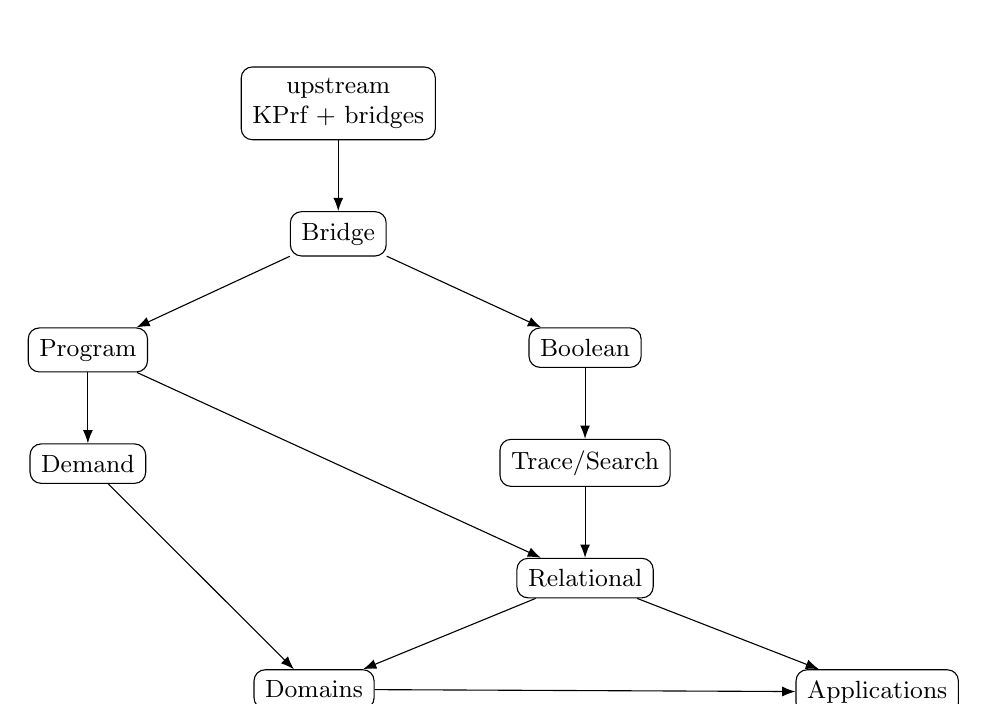
\begin{tikzpicture}[node distance=9mm and 18mm, every node/.style={draw,rounded corners,align=center,inner sep=4pt,font=\small}, >=Latex]
\node (up) {upstream\\KPrf + bridges};
\node (bridge) [below=of up] {Bridge};
\node (program) [below left=of bridge] {Program};
\node (bool) [below right=of bridge] {Boolean};
\node (trace) [below=of bool] {Trace/Search};
\node (demand) [below=of program] {Demand};
\node (rel) [below=of trace] {Relational};
\node (domain) [below left=of rel] {Domains};
\node (apps) [below right=of rel] {Applications};
\draw[->] (up) -- (bridge);
\draw[->] (bridge) -- (program);
\draw[->] (bridge) -- (bool);
\draw[->] (bool) -- (trace);
\draw[->] (program) -- (demand);
\draw[->] (program) -- (rel);
\draw[->] (trace) -- (rel);
\draw[->] (demand) -- (domain);
\draw[->] (rel) -- (domain);
\draw[->] (domain) -- (apps);
\draw[->] (rel) -- (apps);
\end{tikzpicture}
\end{center}

The archive includes files with these names.  \path{Bridge.lean} is written as
candidate direct code using current upstream declarations.  The other files are
blueprints with explicit theorem signatures and \path{sorry}; they are not
presented as compiled modules.

\subsection{Bridge module}

The first module should prove only four small theorems:

\begin{enumerate}
\item \path{cutAsmList}: discharge a list of ordinary assumptions using
\path{KPrf.cut};
\item \path{cutOne}: one-output specialization of list cut;
\item \path{exportPRA}: compose \path{KPrf.toNPrf} with
\path{native_iff_pra};
\item \path{importPRA}: compose \path{pra_iff_native} with
\path{kprf_iff_nprf}.
\end{enumerate}

The intended declarations are:

\begin{lstlisting}[language={},caption={Core proof-exchange API}]
theorem cutAsmList
    (h : KPrf (Delta.map Cl.asm ++ Gamma) A)
    (hs : forall X in Delta, KPrf Gamma X) : KPrf Gamma A

theorem exportPRA (h : KPrf Gamma A) :
    Gamma.map (fun c => c.toN.toPRA) |- [PRAAx] A.toPRA

theorem importPRA (h : Gamma |- [PRAAx] phi) :
    KPrf ((Gamma.map NFm.ofPRA).map
      (fun X => Cl.asm (NFm.unQ X)))
      (NFm.unQ (NFm.ofPRA phi))
\end{lstlisting}

The exact notation in the artifact follows upstream syntax.  Because no Lean
binary was present, even these short declarations are labeled ``candidate''
until checked in the repository workspace.

\subsection{Dependent program datatype}

A program should record the earlier outputs available to each node.
One possible datatype is:

\begin{lstlisting}[language={},caption={Suggested dependent schedule}]
structure Node (n : Nat) (Gamma : List (Cl n))
    (available : List (NFm n)) where
  out : NFm n
  local : KPrf (available.map Cl.asm ++ Gamma) out

inductive Program (n : Nat) (Gamma : List (Cl n)) :
    List (NFm n) -> Type
  | nil : Program n Gamma []
  | snoc {outs} : Program n Gamma outs ->
      Node n Gamma outs -> Program n Gamma (node.out :: outs)
\end{lstlisting}

The order of \path{outs} can be newest-first to make extension constant-time.
The compiler returns a proof environment:

\begin{lstlisting}[language={}]
def Compiled (Gamma : List (Cl n)) (outs : List (NFm n)) : Prop :=
  forall A, A in outs -> KPrf Gamma A

theorem Program.compile (p : Program n Gamma outs) :
  Compiled Gamma outs
\end{lstlisting}

The proof is induction on \path{p}; the step is \path{cutAsmList}.  A terminal
method extracts the proof of the newest output.  This theorem should be the
first new kernel-checked milestone, because it validates the architecture with
minimal domain machinery.

\subsection{Sparse dependencies}

For large graphs, a node should not assume every previous output.  Store a list
of indices \path{deps : List (Fin available.length)} and define the dependency
formula list by lookup.  The compiler maps each index to the corresponding
compiled proof.  Correctness is still list cut.

An alternative is a named finite map.  Indices are preferable in the kernel
layer because membership and lookup are structurally simple; human-readable
names belong in generated metadata.

\subsection{Formula builders}

Application code should not manipulate raw de Bruijn indices everywhere.
Create typed builders for common forms:

\begin{itemize}
\item equations and Boolean equations;
\item bounded predicates compiled to characteristic terms;
\item tuple/list access equations;
\item guarded clauses;
\item trace-state invariants;
\item rational error inequalities;
\item relation and observer formulas.
\end{itemize}

Each builder should come with substitution lemmas and, where possible,
\path{simp} theorems.  The builders elaborate to ordinary \(\NFm\) or
\(\mathrm{Fm}\;\PTm\), so they do not enlarge the trusted kernel.

\subsection{Booleanization module}

There are two implementation strategies.

\paragraph{Reuse existing reflection.}
Audit \path{TeqReflect.lean} and related files for characteristic terms and
quantifier-free induction.  Add adapters to the \path{IPRADerivations} term
symbols and native formulas.

\paragraph{A small dedicated AST.}
Define a restricted Boolean formula syntax with equality, not, and, or, and
bounded folds.  Compile it to a PR characteristic term and to an ordinary
formula, then prove equivalence by structural induction.  This is easier to use
for generated verifiers and avoids proving reflection for arbitrary syntax.

The second route is recommended for the first milestone.  General reflection
can be integrated later.

\subsection{Trace module}

A direct ordinary-iPRA API can build on \path{IPRADerivations.ind}:

\begin{lstlisting}[language={}]
structure TraceSpec (k : Nat) where
  state : PTm (k + 1)
  inv : Fm PTm (k + 1)
  qf : inv.QF
  base : [] |- [PRAAx] inv.subst (inst zero)
  step : [inv] |- [PRAAx] inv.subst (repl (succ (var 0)))

theorem TraceSpec.closed (S : TraceSpec k) :
  [] |- [PRAAx] S.inv := ind S.inv S.qf S.base S.step
\end{lstlisting}

A higher-level builder constructs the state term from an initializer and step
PR symbol and constructs \path{base} and \path{step} from local equations.
Search, bounded folds, table construction, and demand passes are specializations.

\subsection{Demand module}

The pure metatheoretic layer can first be implemented over
\path{Vector Nat k} or \path{Fin k -> Nat} to prove the finite lattice theorems.
The object layer then chooses a concrete tuple code and PR functions.  Required
theorems are:

\begin{enumerate}
\item componentwise order and join laws;
\item rank strictness for a strict componentwise increase;
\item bounded closure termination;
\item fixed-point and leastness;
\item reverse DAG propagation correctness and minimality;
\item schedule lookup and replay correctness.
\end{enumerate}

Do not stop at the metatheoretic theorem.  The endpoint is a
\(\Prf\;\PRAAx\) trace theorem for the encoded closure algorithm.  The
metatheory guides the proof and tests the definitions.

\subsection{Relational module}

Define bounded clouds by a bound and Boolean predicate rather than by Mathlib
finite sets.  This representation maps directly to PR terms.  The module should
provide:

\begin{itemize}
\item reverse viability table;
\item least viable witness and least successor;
\item path coding and edge correctness;
\item exact observer invariance;
\item rational diameter check;
\item motion-tail Cauchy estimate;
\item gap-based exact recovery.
\end{itemize}

The general theorems should be proved once in ordinary iPRA and imported into
the native graph as needed.

\subsection{Algebra-node import}

A small adapter should turn an \path{IPRADerivations} theorem into a native node.
For a direct theorem \path{h}, define the node output to be
\path{NFm.unQ (NFm.ofPRA phi)} and the local proof to be
\path{importPRA h}.  The node's predecessor formulas are the translations of
\path{h}'s assumptions.

The reverse adapter exports a terminal node with \path{exportPRA}.  Round-trip
theorems can be used to rewrite the result to the human-facing formula rather
than leaving a translated formula in the public API.

\subsection{Suggested completion sequence}

\begin{longtable}{L{0.09\textwidth}L{0.42\textwidth}L{0.39\textwidth}}
\toprule
Step & Deliverable & Acceptance criterion \\
\midrule
1 & \path{Bridge.lean} & Compiles; no \path{sorry}; axiom audit no stronger than upstream metatheory.\\
2 & \path{Program.lean} & A two-node and a five-node graph compile to closed \(\KPrf\) proofs.\\
3 & Algebra exchange demo & Import one checked Heron-related identity, compose a native equality node, export to the same ordinary formula.\\
4 & Boolean formulas & Characteristic-term compiler for the restricted verifier language, with object-level equivalence.\\
5 & Trace and search & Closed derivations for a counter trace, least bounded search, and complete enumeration.\\
6 & Demand & Object-level finite monotone closure and a small cyclic example.\\
7 & Relational & Object-level three-layer viability and stable observer example.\\
8 & Domain library & Rational arithmetic, finite lists/tables, and dyadic errors.\\
9 & Packet migration & Convert one existing proof packet end to end, keeping a claim ledger.\\
10 & Automation & Generate node syntax and proof schedules from a declarative JSON or Lean DSL.\\
\bottomrule
\end{longtable}

\subsection{Testing and axiom audits}

Every checked theorem module should have an audit file using \path{#print axioms}
or the repository's established mechanism.  Every generated graph should have:

\begin{itemize}
\item a small executable reference example;
\item a test that deliberately corrupts one local certificate and is rejected;
\item a theorem statement snapshot to detect accidental weakening;
\item a count of \path{sorry}, expected to be zero in checked modules;
\item a comparison between the public ordinary formula and the exported
translation.
\end{itemize}

The proof kernel, not the tests, remains the authority.  Tests protect the code
generator and theorem statement.

\subsection{Avoiding common Lean traps}

\begin{enumerate}
\item Do not define the main theorem as a structure field and then count the
structure constructor as a proof.
\item Do not use a host theorem \path{eval spec = true} as the final endpoint
unless a proved reflection theorem constructs the object derivation.
\item Keep semantic interpretations and syntactic derivations in different
namespaces.
\item Normalize contexts before invoking bridge theorems; most failures are
list-map or \path{unQ} mismatches.
\item Prefer checked structural lemmas to rewriting under binders by hand.
\item Expose all conditional producer assumptions in the public theorem type.
\item Pin the upstream commit because the native calculus is under active
research and names may change.
\end{enumerate}

\section{Executable evidence, reproducibility, and claim discipline}

\subsection{Reference implementation}

The archive contains \path{code/native_clause_framework.py}.  It implements,
with exact integer and rational arithmetic:

\begin{itemize}
\item bounded least search and complete enumeration;
\item least closure of a monotone transformer on a finite product of chains;
\item exhaustive monotonicity checks for small test boxes;
\item reverse demand propagation on a DAG;
\item clocked trace execution and invariant checking;
\item backward relational viability and least viable paths;
\item stable-observer diameter checks and motion tails;
\item exact label recovery from a separation gap;
\item conversion between a height bound and a finite list;
\item common good windows for finite exceptional sets;
\item lexicographic descent fuel;
\item execution of a finite contract graph with local host-level checkers.
\end{itemize}

The final item is deliberately documented as an executable analogue, not an
object proof.  The distinction is enforced in the module docstring.

\subsection{Regression tests}

The accompanying test suite has fourteen tests.  It covers success and failure
cases, exact rational stability, cyclic demand closure, demand minimality in a
small graph, trace invariants, relational failure, gap recovery, and graph
certificate rejection.  The recorded run in
\path{validation/python_tests.txt} reports all tests passing.

These tests provide three kinds of evidence:

\begin{enumerate}
\item the finite algorithms are specified precisely enough to execute;
\item examples in the report match the implementation;
\item later refactoring can detect changes in behavior.
\end{enumerate}

They do not prove the general theorems and do not check the Lean outline.

\subsection{Machine-readable schema}

\path{schema/native_clause_program.schema.json} describes a declarative program
format.  A node records its identifier, kind, dependencies, output formula
name, demand/resource metadata, and the provenance of its local proof.  The
schema does not serialize Lean proof terms.  It is intended for generators and
audits: the generated Lean source must still be elaborated and kernel-checked.

\subsection{Theorem ledger}

\path{metadata/THEOREM_LEDGER.md} classifies every main result as one of:

\begin{itemize}
\item \textbf{upstream checked}: a theorem already present in the pinned
repository;
\item \textbf{human complete}: a proof is given in this report;
\item \textbf{executable evidence}: exact reference code and tests exist;
\item \textbf{Lean candidate}: code is supplied but not compiled here;
\item \textbf{blueprint}: definitions and theorem signatures give a clear path,
with proof holes explicitly counted;
\item \textbf{conditional/application-specific}: the generic finalizer is
proved but a deep producer is not supplied.
\end{itemize}

This vocabulary is intentionally conservative.  ``Formalized'' is reserved for
kernel-checked source in the target calculus.

\subsection{Source provenance}

The source audit records:

\begin{itemize}
\item the pinned repository commit;
\item paths and blob hashes of the key upstream files;
\item the status statement in the parent iPRA README;
\item the earlier foundation packets compared;
\item the newly added direct derivation library;
\item the exact absence of Lean executables in the artifact environment.
\end{itemize}

The build does not download dependencies.  It compiles the PDF, runs the Python
tests, produces the demo JSON, and refreshes checksums.  Lean checking must be
performed in the pinned ProveIt workspace.

\subsection{PDF validation}

The report is compiled twice with \path{pdflatex}, inspected with
\path{pdfinfo}, preflighted, rendered to PNG at high resolution, and sampled
across the document for visual defects.  The validation directory records page
count, metadata, preflight output, and the pages inspected.  Intermediate
renders are not included in the final ZIP.

\subsection{Negative claims}

This package does not claim:

\begin{itemize}
\item that its new Lean files compile;
\item that the Python program is an iPRA proof checker;
\item that every proof packet in the repository is correct;
\item a universal primitive-recursive evaluator;
\item a general effective proof of Faltings, Siegel, or every stated
prime-distribution theorem;
\item a canonical selector for singular roots, spectra, quotient
representatives, or compatible infinite paths;
\item that classical finiteness by itself yields a search cutoff;
\item that a semantic Lean theorem is interchangeable with
\(\Prf\;\PRAAx\).
\end{itemize}

The positive claim is narrower and more actionable: current checked
\path{ConciseIPRA} already exposes a proof language in which a genuine generic
finite graph compiler can be very small, and the current checked direct
arithmetic library can exchange theorems with that compiler.

\section{Conclusion}

The repository's finitary proof packets have largely converged on the right
mathematical ideas: finite observations, explicit moduli and resource bounds,
clocked recursion, bounded search, relational witnesses, and stable outputs.
The main remaining difficulty is no longer conceptual breadth.  It is proof
composition in the actual embedded calculus.

The native clause calculus \(\KPrf\) supplies the missing intermediate
representation.  Its checked substitution theorem specializes local contracts;
its checked cut theorem composes a finite graph; its translation to
\(\NPrf\) and the checked native/iPRA equivalence export the result to ordinary
\(\Prf\;\PRAAx\).  The newly checked \path{IPRADerivations} library supplies a
second backend for symbolic arithmetic and polynomial identities, and the
bridges run in both directions.

The proposed workflow is therefore concrete:

\begin{enumerate}
\item formulate the theorem as finite observation contracts;
\item make every modulus, height, gap, cover, fuel, and threshold explicit;
\item prove local algebra directly in \(\Prf\;\PRAAx\);
\item prove local control contracts in \(\KPrf\);
\item retain unstable data as bounded relations and observe only stable
information;
\item compute demands, including cyclic closure, in a bounded finite effect
system;
\item fold the graph by checked cut and export the terminal theorem.
\end{enumerate}

This architecture resolves the generic encoding and composition problems while
leaving deep mathematics where it belongs: in explicit producer theorems.
That boundary is a strength.  It makes completed results genuinely checkable
and makes remaining obstacles precise enough to attack one at a time.

The highest-value next step is not another broad packet.  It is a small checked
implementation of \path{Bridge.lean} and \path{Program.lean}, followed by one
end-to-end example that imports an existing \path{ipra_ring} theorem, composes a
bounded trace or search node, and exports the exact ordinary iPRA sentence.  A
successful example would turn the present framework from a detailed blueprint
into shared infrastructure for the entire proof corpus.

\appendix
\section{Theorem catalog and dependency map}

This appendix lists the generic results in dependency order.  ``Upstream'' means
that the named theorem already occurs in the pinned repository.  ``Report''
means that a complete human proof is given here and a Lean target is specified.

\begin{longtable}{L{0.08\textwidth}L{0.30\textwidth}L{0.16\textwidth}L{0.35\textwidth}}
\toprule
ID & Result & Status & Dependencies and role \\
\midrule
U1 & \path{KPrf.subst} & Upstream checked & Specializes local native proofs and clause contexts.\\
U2 & \path{KPrf.cut} & Upstream checked & Discharges retained or proved assumption clauses.\\
U3 & \path{KPrf.toNPrf} & Upstream checked & Maps clause derivations to native scalar-core derivations.\\
U4 & \path{kprf_iff_nprf} & Upstream checked & Completeness/equivalence after \path{unQ}.\\
U5 & \path{native_iff_pra} & Upstream checked & Exports native proofs to ordinary iPRA.\\
U6 & \path{pra_iff_native} & Upstream checked & Imports ordinary iPRA proofs into the native core.\\
U7 & \path{IPRADerivations.ind} & Upstream checked & Open quantifier-free induction.\\
U8 & \path{IPRADerivations.inst} & Upstream checked & Instantiates closed direct derivations.\\
U9 & \path{ipra_ring} & Upstream checked tactic & Generates polynomial identity derivations.\\
C1 & List cut & Report, Lean candidate & U2; discharges a list of generated assumptions.\\
C2 & Native DAG compilation & Report, blueprint & C1; topological fold of local \(\KPrf\) proofs.\\
C3 & Clause-to-iPRA export & Report, Lean candidate & U3 and U5.\\
C4 & iPRA-to-clause import & Report, Lean candidate & U6 and U4.\\
B1 & QF Booleanization & Report, blueprint & Structural syntax recursion; bounded folds.\\
B2 & Finite trace reflection & Report, blueprint & B1 and U7.\\
B3 & Least bounded search & Report, executable & B2 and B1.\\
B4 & Complete bounded enumeration & Report, executable & B2 and B1.\\
B5 & Finite lexicographic fuel & Report, executable & Mixed-radix rank.\\
B6 & Common good finite window & Report, executable & Finite union bound and B3.\\
D1 & Least acyclic demand & Report, executable & Reverse topological induction.\\
D2 & Finite monotone closure & Report, executable & Rank sum on product of chains.\\
D3 & Scheduled recurrence & Report, blueprint & D1/D2, B2, C2.\\
R1 & Backward viability & Report, executable & Reverse Boolean dynamic program and B3.\\
R2 & Exact observer elimination & Report, blueprint & R1 and bounded invariance.\\
R3 & Approximate observer elimination & Report, executable & R1 and rational diameter.\\
R4 & Motion-tail Cauchy bound & Report, executable & Finite triangle inequality.\\
R5 & Gap-based exact recovery & Report, executable & Separation and B3.\\
H1 & Height--list conversion & Report, executable & B4 and finite maximum.\\
P1 & Producer--verifier--finalizer factorization & Design theorem & C2, explicit interfaces.\\
\bottomrule
\end{longtable}

\subsection{Minimal trusted path for a closed theorem}

For a closed terminal formula \(A\), the proposed new code contributes only the
program fold and bridge composition:
\[
\begin{array}{c}
  h_i:\KPrf(\text{predecessor assumptions},A_i)\\[2mm]
  \Downarrow\;\text{C1, C2}\\[2mm]
  h:\KPrf([],A)\\[2mm]
  \Downarrow\;\text{U3}\\[2mm]
  \NPrf([],A)\\[2mm]
  \Downarrow\;\text{U5}\\[2mm]
  []\vdash_{\PRAAx}A.\mathsf{toPRA}.
\end{array}
\]
All domain-specific computation occurs in the local proofs \(h_i\).  The
compiler itself does not evaluate formulas or assert their truth.

\subsection{Suggested first checked theorem}

A useful smoke theorem is a two-node program.  Node 0 derives a simple iterator
equation.  Node 1 assumes that equation and derives its symmetric form using a
checked equality lemma.  The program compiler should derive the symmetric form
from the empty context.  Export should produce a closed iPRA equality.  This
example exercises clause assumptions, cut, and the bridge without requiring a
new coding library.

The second theorem should import one existing direct polynomial identity,
compose it with a native substitution/equality node, and export it.  This tests
the two-backend exchange.

\section{Reusable proof templates}

\subsection{Template: deterministic numerical operation}

\textbf{Data.}
PR terms \(f\) and \(d\), input validity formula \(V_X(x,d(q),o)\), output
validity formula \(V_Y(f(x),q,f_o(x,q,o))\).

\textbf{Local theorem.}
A \(Q\)-free native derivation of
\[
    V_X(x,d(q),o)\to V_Y(f(x),q,f_o(x,q,o)).
\]
Encode the implication as a clause or import its ordinary derivation.

\textbf{Graph use.}
The predecessor node exports input validity.  Specialize the local theorem at
the concrete terms.  List cut discharges the predecessor assumption.

\subsection{Template: guarded division}

\textbf{Data.}
Rational codes \(a,b\), a guard \(G(b,g)\) certifying
\(|b|\ge2^{-g}\), and requested precision \(q\).

\textbf{Demand.}
Choose \(r=q+c(g,M_a,M_b)\) so that input errors preserve
\(|b_r|\ge2^{-g-1}\) and the reciprocal error is below the budget.

\textbf{Verifier.}
Check denominator positivity, the rational lower bound, and the final cleared-
denominator error inequality.

\textbf{Output.}
A rational code \(a_r/b_r\) and an error certificate.  The totalized function
returns zero if the guard fails; the correctness clause has \(G\) as
antecedent.

\subsection{Template: bounded search with negative result}

\textbf{State.}
Clock, found flag, least witness, and Boolean prefix verifier.

\textbf{Invariant.}
If found, the witness is below the clock, satisfies the predicate, and all
smaller candidates fail.  If not found, every candidate below the clock fails.

\textbf{Output.}
A disjoint finite result: \path{found(w)} or \path{none}, each with its exact
contract.  Do not use a sentinel value without a status flag.

\subsection{Template: finite descent}

\textbf{Data.}
A fixed-dimensional bounded measure \(m(s)\), a step that either halts or
strictly lowers the measure, and a bound vector \(B\).

\textbf{Fuel.}
Use the mixed-radix state count \(\prod_i(B_i+1)\), or a sharper rank bound.

\textbf{Invariant.}
The current state is valid; the measure lies in the box; every nonhalt step
strictly lowers rank; once halted, the result is preserved.

\textbf{Conclusion.}
The trace halts within the fuel and the terminal certificate is valid.

\subsection{Template: cyclic precision contract}

\textbf{Data.}
A finite box \(L\), monotone demand transformer \(F\), and initial request
\(a\).

\textbf{Algorithm.}
Iterate \(x\mapsto x\join F(x)\) for
\(1+\sum_i(B_i-a_i)\) steps, recording a failure if \(F(x)\notin L\).

\textbf{Invariant.}
The sequence is monotone, remains in the box, and is below every prefixed point
above \(a\).

\textbf{Conclusion.}
Either a least closed demand is returned or a resource-coordinate overflow is
certified.

\subsection{Template: relational cloud}

\textbf{Data.}
Finite bounds \(B(q)\), validity \(G(q,w)\), and edge relation \(E(q,w,v)\).

\textbf{Algorithm.}
Build viability tables backward; select a least finite path only if a concrete
path is needed.

\textbf{Observer.}
Supply exact invariance, a diameter bound, or a motion-tail bound.  Export the
observer, not the implementation path.

\textbf{Exact labels.}
Add a finite label family and a positive separation certificate, then use
Theorem~\ref{thm:gap}.

\subsection{Template: certificate-only theorem}

\textbf{Producer interface.}
A code \(c\) and a bounded checker \(\mathsf{ok}(x,c)=1\).

\textbf{Soundness theorem.}
A local object derivation of
\[
       \mathsf{ok}(x,c)=1\to\Phi(x,\mathsf{out}(c)).
\]

\textbf{Completeness options.}
Either prove a PR producer \(p(x)\) with \(\mathsf{ok}(x,p(x))=1\), accept
\(c\) as explicit input/hypothesis, or state a bounded relation of all accepted
certificates.  Do not infer completeness from successful tests.

\subsection{Template: finite local-to-global argument}

\textbf{Data.}
A coded finite cover, local observations, overlap graph, and compatibility
clauses.

\textbf{Control.}
Use a spanning tree or finite nerve traversal.  At each edge, transport the
local invariant.  Cycles are checked by bounded commutativity conditions.

\textbf{Global output.}
A glued observation or stable quotient class.  A unique global representative
requires a separate uniqueness theorem; otherwise retain the equivalence class.

\subsection{Template: direct algebra plus control}

\textbf{Algebra phase.}
Use \path{ipra_ring} or a direct \(\Prf\;\PRAAx\) lemma to prove an open
identity.

\textbf{Import.}
Apply Theorem~\ref{thm:import} and store the resulting native formula as a node.

\textbf{Control phase.}
Use bounded cases, search, or a trace in \(\KPrf\), specializing the algebra
node as needed.

\textbf{Export.}
Apply Theorem~\ref{thm:export}, then use round-trip equivalence to present the
ordinary formula in its original syntax.

\section{Source audit and comparison with prior frameworks}

\subsection{Pinned repository state}

The research audit used ProveIt commit
\path{8649990597d73657bde480b6c389de7f85bc0cb0}, committed on
16 November 2026 UTC, which is still 15 November in America/Los\_Angeles at the
time of this work.  The commit itself concerns another project, but includes the
recently placed iPRA framework packets and the new direct derivation library
from preceding commits.

Key source files and roles are:

\begin{longtable}{L{0.48\textwidth}L{0.43\textwidth}}
\toprule
Path & Audited role \\
\midrule
\path{Logic/PrimitiveRecursiveArithmetic/README.md} & Defines iPRA used by the repository and records that proof packets were filed without verification.\\
\path{ConciseIPRA/Lean/ConciseIPRA/NativeClausal.lean} & Defines \(\NFm.\mathsf{QFree}\), \path{unQ}, clauses, and the raw clause calculus.\\
\path{ConciseIPRA/Lean/ConciseIPRA/NativeClausalDiagonal.lean} & Defines \(\KPrf\); proves substitution, cut, soundness to \(\NPrf\), and equivalence with the native kernel.\\
\path{ConciseIPRA/Lean/ConciseIPRA/NativeBiInterpretation.lean} & Defines \path{NFm.toPRA}, \path{NFm.ofPRA}, \path{native_iff_pra}, \path{pra_iff_native}, and round trips.\\
\path{Derivations/README.md} & States the checked status and architecture of direct theorem derivations.\\
\path{Derivations/Lean/IPRADerivations/Core/Basic.lean} & Arithmetic symbols, equations, congruence, \path{ind}, and \path{inst}.\\
\path{Derivations/Lean/IPRADerivations/Core/Tactic.lean} & Universal closure and \path{ipra_ring}.\\
\path{docs/proofs/foundations/ocipra_framework_2026-11-15} & Observation contracts, theorem classes, demand closure, and producer/verifier distinctions.\\
\path{docs/proofs/foundations/ipra_pfig_framework_2026-11-15} & Backward-demand/forward-execution proof graphs and compiler blueprint.\\
\path{docs/proofs/foundations/ipra_proof_carrying_observation_graphs_2026-11-15} & Proof-carrying node architecture, relational paths, and stable observers.\\
\bottomrule
\end{longtable}

\subsection{What is reused}

This report reuses the finite-observation and explicit-resource discipline of
the earlier packets.  In particular, it retains:

\begin{itemize}
\item deterministic, relational, stable-observer, and conditional theorem
classes;
\item backward precision demand and forward replay;
\item bounded trace reflection and relational viability;
\item the separation between producers, verifiers, and finalizers;
\item the warning that cardinality is not a height bound;
\item strict separation of semantic host theorems from object derivations.
\end{itemize}

These ideas are not rebranded as new discoveries.

\subsection{What is new in the present synthesis}

The principal new synthesis is to use the current five-rule \(\KPrf\) clause
calculus as the compiler intermediate representation and to connect it
bidirectionally with the newly checked direct derivation backend.  Earlier
packets generally target \(\Prf\;\PRAAx\) directly or define their own contract
structures.  The present design observes that:

\begin{enumerate}
\item graph composition is exactly \path{KPrf.cut};
\item specialization is exactly \path{KPrf.subst};
\item arbitrary native formulas can be normalized by \path{unQ};
\item export is \path{KPrf.toNPrf} followed by \path{native_iff_pra};
\item direct polynomial derivations can be imported by
\path{pra_iff_native} and \path{kprf_iff_nprf}.
\end{enumerate}

This does not by itself complete the Lean compiler, but it removes most of its
logical burden and gives a sharply bounded implementation project.

\subsection{Environment audit}

The artifact environment contained Python, \path{pdflatex}, \path{latexmk},
\path{pdftoppm}, and PDF inspection tools.  It did not contain \path{lean} or
\path{lake}.  No Lean compilation is therefore claimed.  The package includes
candidate source and a completion plan, and all status files repeat this
limitation.

\subsection{Reproducibility}

From the package root:

\begin{lstlisting}[language={}]
python3 verify.py
./build.sh
\end{lstlisting}

The first command runs standard-library Python tests and checks the manifest.
The second runs tests, regenerates the demo, compiles the PDF, records metadata,
and refreshes checksums.  The build is offline and does not modify the ProveIt
repository.


\begingroup
\small
\setlength{\parskip}{0pt}
\begin{thebibliography}{30}
\setlength{\itemsep}{0.25em}
\bibitem{ProveItPRA}
V.~Reshetnikov, \emph{Primitive recursive arithmetic},
\path{Logic/PrimitiveRecursiveArithmetic/README.md}, ProveIt repository,
commit \path{8649990597d73657bde480b6c389de7f85bc0cb0}, 2026.

\bibitem{ConciseIPRA}
V.~Reshetnikov, \emph{Concise presentations of intuitionistic primitive recursive arithmetic},
\path{Logic/PrimitiveRecursiveArithmetic/ConciseIPRA}, ProveIt repository, 2026.

\bibitem{NativeClausal}
V.~Reshetnikov, \emph{Five rules, closed under substitution},
\path{ConciseIPRA/Lean/ConciseIPRA/NativeClausalDiagonal.lean}, 2026.

\bibitem{NativeBi}
V.~Reshetnikov, \emph{Bi-interpretability of the native scalar core with iPRA},
\path{ConciseIPRA/Lean/ConciseIPRA/NativeBiInterpretation.lean}, 2026.

\bibitem{Derivations}
V.~Reshetnikov, \emph{iPRA derivations of theorems from the proof packets},
\path{Logic/PrimitiveRecursiveArithmetic/Derivations}, 2026.

\bibitem{OCiPRA}
\emph{OCiPRA: Observation-Contract Internalization for iPRA},
\path{docs/proofs/foundations/ocipra_framework_2026-11-15}, 2026.

\bibitem{PCOG}
\emph{Proof-Carrying Observation Graphs for iPRA},
\path{docs/proofs/foundations/ipra_proof_carrying_observation_graphs_2026-11-15}, 2026.

\bibitem{PFIG}
\emph{Proof-Producing Finitary Interface Graphs for iPRA},
\path{docs/proofs/foundations/ipra_pfig_framework_2026-11-15}, 2026.

\bibitem{ProofIndex}
V.~Reshetnikov, \emph{iPRA proof-packet index},
\path{Logic/PrimitiveRecursiveArithmetic/docs/proofs/README.md}, 2026.
\end{thebibliography}
\endgroup
\end{document}
